\documentclass[12pt]{article}


\usepackage[margin=1.1in,footskip=.25in]{geometry}

\usepackage{tabularx}
\usepackage[table]{xcolor}
\usepackage{multirow}

\usepackage{listings}
\usepackage{xcolor}
\usepackage{color}

\usepackage{verbatim}

\definecolor{dkgreen}{rgb}{0,0.6,0}
\definecolor{gray}{rgb}{0.5,0.5,0.5}
\definecolor{mauve}{rgb}{0.58,0,0.82}
 
\definecolor{codegreen}{rgb}{0,0.6,0}
\definecolor{codegray}{rgb}{0.5,0.5,0.5}
\definecolor{codepurple}{rgb}{0.58,0,0.82}
\definecolor{backcolour}{rgb}{0.95,0.95,0.92}



\lstdefinestyle{mystyle}{
    commentstyle=\color{codegreen},
    keywordstyle=\color{magenta},
    numberstyle=\tiny\color{codegray},
    stringstyle=\color{codepurple},
    basicstyle=\ttfamily\normalsize,
    breakatwhitespace=false,         
    breaklines=true,                 
    captionpos=b,                    
    keepspaces=true,                              
    showspaces=false,                
    showstringspaces=false,
    showtabs=false,                  
    tabsize=3
}

\lstset{style=mystyle}

\newcolumntype{C}{ >{\centering\arraybackslash} m{5cm} }
\newcolumntype{E}{ >{\centering\arraybackslash} m{7cm} }
\newcolumntype{D}{ >{\centering\arraybackslash} m{3cm} }
\newcolumntype{F}{ >{\centering\arraybackslash} m{1cm} }

\usepackage{array}

\usepackage{tikz} 
\usetikzlibrary{graphs,quotes,arrows.meta}
\usetikzlibrary{automata}
\usetikzlibrary{positioning}
\usetikzlibrary{patterns}
\usetikzlibrary{matrix,backgrounds}
\usetikzlibrary{arrows,shapes,trees}
\usetikzlibrary{chains}
\usetikzlibrary{calc}


\tikzstyle{vertex}=[draw,fill=black!5,circle,minimum size=20pt,inner sep=1pt]
\tikzstyle{error}=[fill=red!60]

\tikzset{
  treenode/.style = {align=center, inner sep=0pt, text centered,
    font=\sffamily},
  arn_n/.style = {treenode, circle, white, font=\sffamily\bfseries, draw=black,
    fill=black, text width=1.5em},% arbre rouge noir, noeud noir
  arn_r/.style = {treenode, circle, red, draw=red,
    text width=1.5em, very thick},% arbre rouge noir, noeud rouge
  arn_x/.style = {treenode, rectangle, draw=black, fill = black,
    minimum width=0.5em, minimum height=0.5em}% arbre rouge noir, nil
}

\usepackage{amsmath, amssymb}
\usepackage{mathtools}
\makeatletter
\def\env@cases{%
  \let\@ifnextchar\new@ifnextchar
  \left\lbrace
  \def\arraystretch{1.2}%
  \array{l@{\quad}l@{}}% Formerly @{}l@{\quad}l@{}
}
\makeatother



\usepackage[most]{tcolorbox}

\tcbset{
    frame code={}
    center title,
    left=10pt,
    right=10pt,
    top=10pt,
    bottom=10pt,
    colback=gray!5,
    colframe=gray,
    width=\dimexpr\textwidth\relax,
    enlarge left by=0mm,
    boxsep=5pt,
    arc=0pt,outer arc=0pt,
}

\usepackage{xepersian}
\settextfont[Scale=1]{Vazir}

\renewcommand{\baselinestretch}{1.3} 

\begin{document}

\tableofcontents

\newpage



\section{درخت
قرمز-مشکی ( \lr{Red-Black} )
}

\begin{latin}
\begin{center}
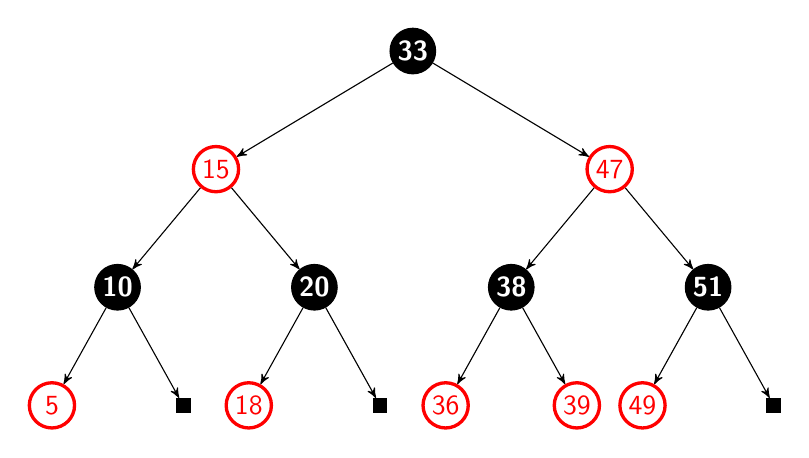
\begin{tikzpicture}[->,>=stealth',level/.style={sibling distance = 5cm/#1,
  level distance = 1.5cm}] 
\node [arn_n] {33}
    child{ node [arn_r] {15} 
            child{ node [arn_n] {10} 
            	child{ node [arn_r] {5}} %for a named pointer
							child{ node [arn_x] {}}
            }
            child{ node [arn_n] {20}
							child{ node [arn_r] {18}}
							child{ node [arn_x] {}}
            }                            
    }
    child{ node [arn_r] {47}
            child{ node [arn_n] {38} 
							child{ node [arn_r] {36}}
							child{ node [arn_r] {39}}
            }
            child{ node [arn_n] {51}
							child{ node [arn_r] {49}}
							child{ node [arn_x] {}}
            }
		}
; 
\end{tikzpicture}
\end{center}
\end{latin}




\subsection {
ویژگی های درخت قرمز-مشکی ( \lr{Red-Black} )
}


\begin{enumerate}
	\item یک درخت جستجوی دودویی متوازن از نظر ارتفاع می باشد .
	\item هر نود به رنگ قرمز یا مشکی می باشد .
	\item عنصر
	\lr{root}
	در درخت به رنگ مشکی می باشد .
	\item عنصر
	\lr{null}
	یا تهی نیز به رنگ مشکی می باشد .
	\item تعداد عناصر مشکی از هر مسیری از
	\lr{root}
	به سمت برگ ها برابر هست
	\item \lr{Parent}
	و
	\lr{Children}
	نمی توانند هر دو به رنگ قرمز باشند .
	\item نود تازه اضافه شده به رنگ قرمز می باشد .
	\item ارتفاع درخت قرمز-مشکی برابر است با :
	$$ \:\: \log{(n)} \leq h \leq 2 \log{(n)} $$
\end{enumerate}



\section{نحوه ی ساخت درخت قرمز-مشکی}

فرض کنید عناصر 
\begin{center}
\lr{keys : 10, 20, 30, 50, 40, 60, 70, 80, 4, 8}
\end{center}
 را به ترتیب برای ساخت درخت قرمز-مشکی استفاده کنیم .



\begin{tcolorbox}
درج در درخت قرمز-مشکی همانند درخت جستوی دودویی می باشد .

\noindent
وقتی یک نود جدید به درخت قرمز-مشکی اضافه می شود ، آن نود به رنگ قرمز باشد باشد
\end{tcolorbox}

در ابتدا عنصر 
\tikz \node [arn_r]  {$10$} ;
را اضافه می کنیم و این عنصر به رنگ قرمز می باشد .



\begin{latin}
\begin{center}
  \bgroup
  \def\arraystretch{1.5}%
  \begin{tabular}{ D C D C  }
  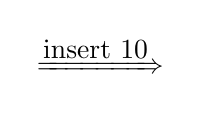
\begin{tikzpicture}
    \draw (0,0) node (arrow) 
{$\xRightarrow{\text{\normalsize insert 10}}$};
\end{tikzpicture} 
  &
    
\begin{tikzpicture}[->,>=stealth',level/.style={sibling distance = 5cm/#1,
  level distance = 1.5cm}] 
\node [arn_r] {10};
\end{tikzpicture}
  \end{tabular}
  \egroup
\end{center}
\end{latin}



از آنجایی که ریشه
(\lr{root})
به رنگ مشکی می باشد عنصر
\tikz \node [arn_r]  {\lr{10}} ;
را به \tikz \node [arn_n]  {$10$} ; تغییر می دهیم .





\begin{latin}
\begin{center}
  \bgroup
  \def\arraystretch{1.5}%
  \begin{tabular}{ D C D C  }
  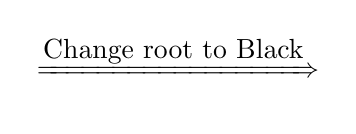
\begin{tikzpicture}
    \draw (0,0) node (arrow) 
{$\xRightarrow{\text{\normalsize Change root to Black}}$};
\end{tikzpicture} 
  &
    
\begin{tikzpicture}[->,>=stealth',level/.style={sibling distance = 5cm/#1,
  level distance = 1.5cm}] 
\node [arn_n] {10};
\end{tikzpicture}
  \end{tabular}
  \egroup
\end{center}
\end{latin}




سپس عنصر 
\tikz \node [arn_r]  {20} ;
را اضافه می کنیم ، به خاطر اینکه این عنصر تازه وارد است به رنگ قرمز می باشد .




\begin{latin}
\begin{center}
  \bgroup
  \def\arraystretch{1.5}%
  \begin{tabular}{ D C D C  }
  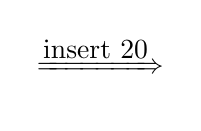
\begin{tikzpicture}
    \draw (0,0) node (arrow) 
{$\xRightarrow{\text{\normalsize insert 20}}$};
    \end{tikzpicture} 
    &
    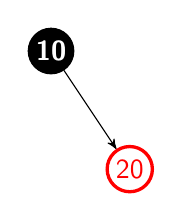
\begin{tikzpicture}[->,>=stealth',level/.style={sibling distance = 2cm,
  level distance = 1.5cm}] 
\node [arn_n] {10}
child [missing] {}
child{
	node [arn_r] {20}
} 
;
\end{tikzpicture}
  \end{tabular}
  \egroup
\end{center}
\end{latin}




سپس عنصر 
\tikz \node [arn_r]  {30} ;
را اضافه می کنیم ، به خاطر اینکه این عنصر تازه وارد است به رنگ قرمز می باشد ، درج این عنصر مشکل 
\textbf{
برخورد قرمزها  
\lr{(red-red conflict)}
}
را به وجود می آورد .




\begin{latin}
\begin{center}
  \bgroup
  \def\arraystretch{1.5}%
  \begin{tabular}{ D C D C  }
  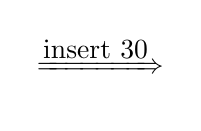
\begin{tikzpicture}
    \draw (0,0) node (arrow) 
{$\xRightarrow{\text{\normalsize insert 30}}$};
    \end{tikzpicture} 
    &
    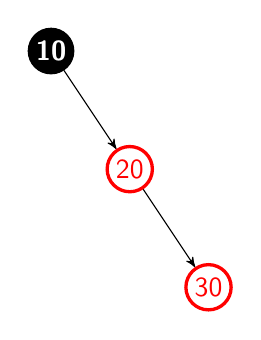
\begin{tikzpicture}[->,>=stealth',level/.style={sibling distance = 2cm,
  level distance = 1.5cm}] 
\node [arn_n] {10}
child [missing] {}
child{
	node [arn_r] {20}
	child [missing] {}
	child{
		node [arn_r] {30}
	} 
} 
;
\end{tikzpicture}
  \end{tabular}
  \egroup
\end{center}
\end{latin}







\begin{tcolorbox}
\textbf{
برخورد قرمزها  
\lr{(red-red conflict)}
}

\noindent
هرگاه برخورد قرمزها پیش بیاید به معنای عدم توازن در درخت قرمز-مشکی می باشد و شما برای برقراری دوباره ی توازن نیاز به تغییراتی در ساختار درخت قرمز-مشکی دارید .


\noindent
دو روش برای انجام تغییرات وجود دارد :

\begin{enumerate}
\item
\text{
تغییر رنگ
\lr{(Re-Coloring)} }
\item
\text{
چرخش
\lr{(Rotation)} }
\end{enumerate}

\end{tcolorbox}


\begin{tcolorbox}
\textbf{
دایی
\lr{(Uncle)}
}

\noindent
برای ادامه ی بحث ما نیاز به آشنایی با یک مفهوم جدید به نام دایی یا
\lr{ Uncle }
داریم که به معنای نودِ همسایه یِ پدر می باشد

\noindent
از این به بعد برای اشاره به این مفهوم از واژه ی 
\lr{ Uncle }
استفاده می کنیم .

\end{tcolorbox}





وقنی برخورد قرمزها به وجود می آید می توانیم 2 حالت نسبت به
\lr{ Uncle }
نود تازه اضافه شده داشته باشیم .


\subsection{
\lr{ Uncle }
قرمز است
}



وقتی
\lr{ Uncle }
نود تازه اضافه شده قرمز باشد ما از روش تغییر رنگ 
\lr{( Re-Coloring )}
استفاده می کنیم .



\begin{latin}
\begin{center}
  \bgroup
  \def\arraystretch{1.5}%
  \begin{tabular}{ C D C  }
    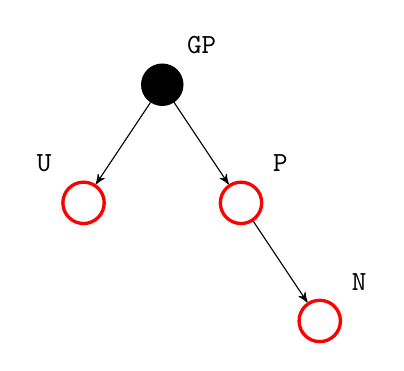
\begin{tikzpicture}[->,>=stealth',level/.style={sibling distance = 2cm,
  level distance = 1.5cm}] 
\node [arn_n] (g) {}
child  {
	node [arn_r] (u) {}
}
child{
	node [arn_r] (p) {}
	child [missing] {}
	child{
		node [arn_r] (n) {}
	} 
} 
;
\node at (g) [xshift=0.5cm,yshift=0.5cm] {\normalsize\ttfamily GP};
\node at (p) [xshift=0.5cm,yshift=0.5cm] {\normalsize\ttfamily P};
\node at (u) [xshift=-0.5cm,yshift=0.5cm] {\normalsize\ttfamily U};
\node at (n) [xshift=0.5cm,yshift=0.5cm] {\normalsize\ttfamily N};
\end{tikzpicture}
    &
    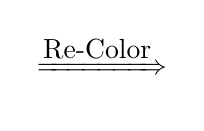
\begin{tikzpicture}
    \draw (0,0) node (arrow) 
{$\xRightarrow{\text{\normalsize Re-Color}}$};
    \end{tikzpicture} 
    &
    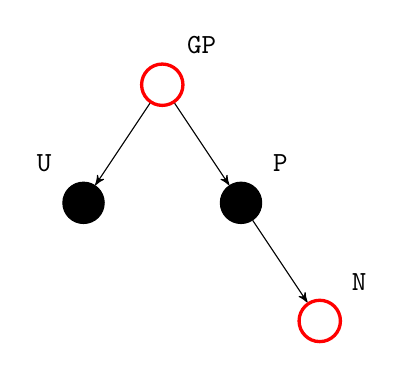
\begin{tikzpicture}[->,>=stealth',level/.style={sibling distance = 2cm,
  level distance = 1.5cm}] 
\node [arn_r] (g) {}
child  {
	node [arn_n] (u) {}
}
child{
	node [arn_n] (p) {}
	child [missing] {}
	child{
		node [arn_r] (n) {}
	} 
} ;
\node at (g) [xshift=0.5cm,yshift=0.5cm] {\normalsize\ttfamily GP};
\node at (p) [xshift=0.5cm,yshift=0.5cm] {\normalsize\ttfamily P};
\node at (u) [xshift=-0.5cm,yshift=0.5cm] {\normalsize\ttfamily U};
\node at (n) [xshift=0.5cm,yshift=0.5cm] {\normalsize\ttfamily N};
\end{tikzpicture}
     \\ 
  \end{tabular}
  \egroup
\end{center}
\end{latin}





در صورتی که بعد از تغییر رنگ ، نود
\lr{(Grand Parent)}
همان ریشه ی درخت بود آن را به رنگ مشکی تغییر می دهیم .



\begin{latin}
\begin{center}
\begin{lstlisting}[language=C++]
if ( GP == root ) {
	Re-Color GP to Black
}
\end{lstlisting}
\end{center}
\end{latin}


\begin{latin}
\begin{center}
  \bgroup
  \def\arraystretch{1.5}%
  \begin{tabular}{ D D C D  }
    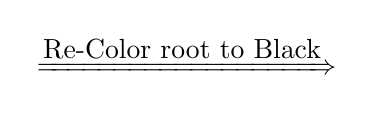
\begin{tikzpicture}
    \draw (0,0) node (arrow) 
{$\xRightarrow{\text{\normalsize Re-Color root to Black}}$};
    \end{tikzpicture} 
    &
    &
    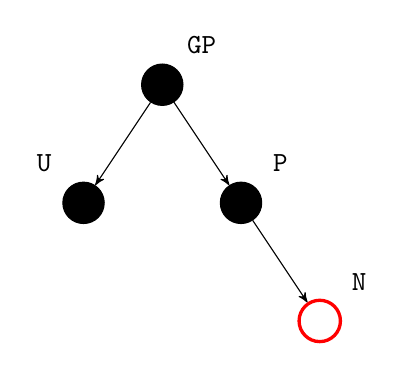
\begin{tikzpicture}[->,>=stealth',level/.style={sibling distance = 2cm,
  level distance = 1.5cm}] 
\node [arn_n] (g) {}
child  {
	node [arn_n] (u) {}
}
child{
	node [arn_n] (p) {}
	child [missing] {}
	child{
		node [arn_r] (n) {}
	} 
} ;
\node at (g) [xshift=0.5cm,yshift=0.5cm] {\normalsize\ttfamily GP};
\node at (p) [xshift=0.5cm,yshift=0.5cm] {\normalsize\ttfamily P};
\node at (u) [xshift=-0.5cm,yshift=0.5cm] {\normalsize\ttfamily U};
\node at (n) [xshift=0.5cm,yshift=0.5cm] {\normalsize\ttfamily N};
\end{tikzpicture}
    
    &
    
     \\ 
  \end{tabular}
  \egroup
\end{center}
\end{latin}



\subsection{
\lr{ Uncle }
مشکی است
}


\subsubsection{حالت اول
\lr{Zig-Zig}}

وقتی
\lr{ Uncle }
نود تازه اضافه شده مشکی باشد ما از روش چرخش 
\lr{ ( Rotation ) }
و در صورت  نیاز از تغییر رنگ 
\lr{ ( Re-Coloring ) }
استفاده می کنیم .



\begin{latin}
\begin{center}
  \bgroup
  \def\arraystretch{1.5}%
  \begin{tabular}{ C D C  }
    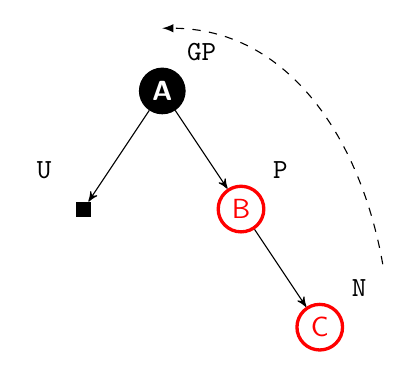
\begin{tikzpicture}[->,>=stealth',level/.style={sibling distance = 2cm,
  level distance = 1.5cm}] 
\node [arn_n] (g) {A}
child  {
	node [arn_x] (u) {}
}
child{
	node [arn_r] (p) {B}
	child [missing] {}
	child{
		node [arn_r] (n) {C}
	} 
} 
;
\node at (g) [xshift=0.5cm,yshift=0.5cm] {\normalsize\ttfamily GP};
\node at (p) [xshift=0.5cm,yshift=0.5cm] {\normalsize\ttfamily P};
\node at (u) [xshift=-0.5cm,yshift=0.5cm] {\normalsize\ttfamily U};
\node at (n) [xshift=0.5cm,yshift=0.5cm] {\normalsize\ttfamily N};

\coordinate (A) at ([yshift=.8cm,xshift=0.8cm]n);
%\coordinate (C) at ([yshift=.5cm,xshift=1cm]r);
\coordinate (C) at ([yshift=.5cm]g.north);

%\draw[dashed] plot[smooth] coordinates {(C) (A)};
\draw[->,>=latex,dashed] (A) to[out=100,in=0] (C);
\end{tikzpicture}
    &
    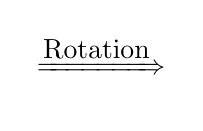
\begin{tikzpicture}
    \draw (0,0) node (arrow) 
{$\xRightarrow{\text{\normalsize Rotation}}$};
    \end{tikzpicture} 
    &
    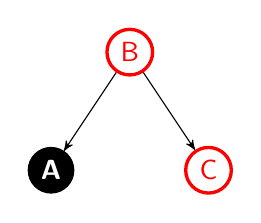
\begin{tikzpicture}[->,>=stealth',level/.style={sibling distance = 2cm,
  level distance = 1.5cm}] 
\node [arn_r] (g) {B}
child  {
	node [arn_n] {A}
}
child{
	node [arn_r] {C}
} 
;
\end{tikzpicture}
     \\ 
  \end{tabular}
  \egroup
\end{center}
\end{latin}





به خاطر اینکه نود ریشه ی درخت قرمز است
آن را به رنگ مشکی تغییر می دهیم .




\begin{latin}
\begin{center}
  \bgroup
  \def\arraystretch{1.5}%
  \begin{tabular}{ C D C  }
    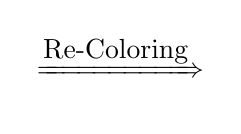
\begin{tikzpicture}
    \draw (0,0) node (arrow) 
{$\xRightarrow{\text{\normalsize Re-Coloring}}$};
    \end{tikzpicture} 
    &
     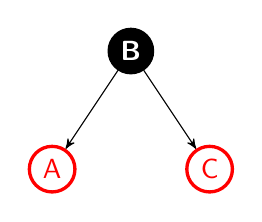
\begin{tikzpicture}[->,>=stealth',level/.style={sibling distance = 2cm,
  level distance = 1.5cm}] 
\node [arn_n] (g) {B}
child  {
	node [arn_r] {A}
}
child{
	node [arn_r] {C}
} 
;
\end{tikzpicture}
    &
    
     \\ 
  \end{tabular}
  \egroup
\end{center}
\end{latin}



\subsubsection{حالت دوم
\lr{Zig-Zag}}





\begin{latin}
\begin{center}
  \bgroup
  \def\arraystretch{1.5}%
  \begin{tabular}{ C D C  }
    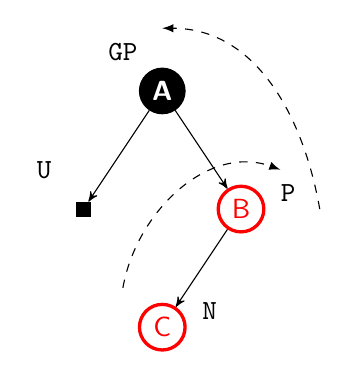
\begin{tikzpicture}[->,>=stealth',level/.style={sibling distance = 2cm,
  level distance = 1.5cm}] 
\node [arn_n] (g) {A}
child  {
	node [arn_x] (u) {}
}
child{
	node [arn_r] (p) {B}
	child{
		node [arn_r] (n) {C}
	} 
	child [missing] {}
} 
;
\node at (g) [xshift=-0.5cm,yshift=0.5cm] {\normalsize\ttfamily GP};
\node at (p) [xshift=0.6cm,yshift=0.2cm] {\normalsize\ttfamily P};
\node at (u) [xshift=-0.5cm,yshift=0.5cm] {\normalsize\ttfamily U};
\node at (n) [xshift=0.6cm,yshift=0.2cm] {\normalsize\ttfamily N};

\coordinate (A) at ([xshift=1cm]p);
\coordinate (C) at ([yshift=.5cm]g.north);

\coordinate (E) at ([yshift=0.5cm,xshift=-0.5cm]n);
%\coordinate (F) at ([yshift=.5cm]a);
\coordinate (G) at ([xshift=0.5cm,yshift=0.5cm]p);

%\draw[dashed] plot[smooth] coordinates {(C) (A)};
\draw[->,>=latex,dashed] (A) to[out=100,in=0] (C);
\draw[->,>=latex,dashed] (E) to[out=80,in=160] (G) ;
\end{tikzpicture}
    &
     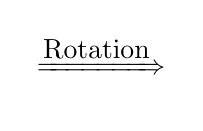
\begin{tikzpicture}
    \draw (0,0) node (arrow) 
{$\xRightarrow{\text{\normalsize Rotation}}$};
    \end{tikzpicture} 
    &
    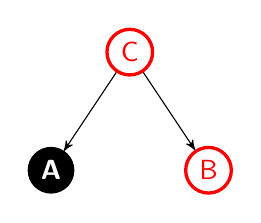
\begin{tikzpicture}[->,>=stealth',level/.style={sibling distance = 2cm,
	  level distance = 1.5cm}] 
	\node [arn_r] (g) {C}
	child  {
		node [arn_n] {A}
	}
	child{
		node [arn_r] {B}
	} 
	;
	\end{tikzpicture}
     \\ 
  \end{tabular}
  \egroup
\end{center}
\end{latin}







به خاطر اینکه نود ریشه ی درخت قرمز است
آن را به رنگ مشکی تغییر می دهیم .





\begin{latin}
\begin{center}
  \bgroup
  \def\arraystretch{1.5}%
  \begin{tabular}{ C D C  }
     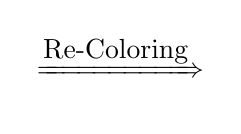
\begin{tikzpicture}
    \draw (0,0) node (arrow) 
{$\xRightarrow{\text{\normalsize Re-Coloring}}$};
    \end{tikzpicture} 
    &
    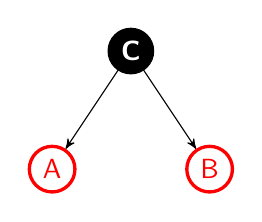
\begin{tikzpicture}[->,>=stealth',level/.style={sibling distance = 2cm,
	  level distance = 1.5cm}] 
	\node [arn_n] (g) {C}
	child  {
		node [arn_r] {A}
	}
	child{
		node [arn_r] {B}
	} 
	;
	\end{tikzpicture}
    &
    
     \\ 
  \end{tabular}
  \egroup
\end{center}
\end{latin}






حالت های زیر نیز می توانند رخ دهند :






\begin{latin}
\begin{center}
  \bgroup
  \def\arraystretch{1.5}%
  \begin{tabular}{ D C C  }
    &
    	Zig-Zig
    &
    Zig-Zag
    \\ \hline
    \\
    &
    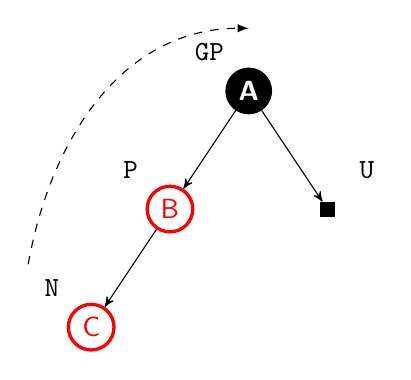
\begin{tikzpicture}[->,>=stealth',level/.style={sibling distance = 2cm,
  level distance = 1.5cm}] 
\node [arn_n] (g) {A}
child{
	node [arn_r] (p) {B}
	child{
		node [arn_r] (n) {C}
	} 
	child [missing] {}
} 
child  {
	node [arn_x] (u) {}
}
;
\node at (g) [xshift=-0.5cm,yshift=0.5cm] {\normalsize\ttfamily GP};
\node at (p) [xshift=-0.5cm,yshift=0.5cm] {\normalsize\ttfamily P};
\node at (u) [xshift=0.5cm,yshift=0.5cm] {\normalsize\ttfamily U};
\node at (n) [xshift=-0.5cm,yshift=0.5cm] {\normalsize\ttfamily N};

\coordinate (A) at ([yshift=.8cm,xshift=-0.8cm]n);
%\coordinate (C) at ([yshift=.5cm,xshift=1cm]r);
\coordinate (C) at ([yshift=.5cm]g.north);

%\draw[dashed] plot[smooth] coordinates {(C) (A)};
\draw[->,>=latex,dashed] (A) to[out=80,in=180] (C);
\end{tikzpicture}
    &
      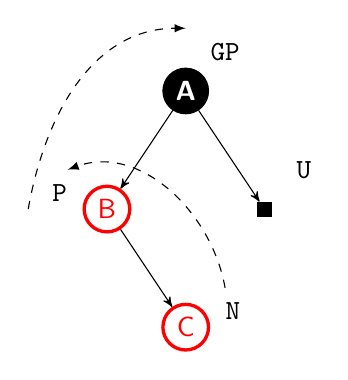
\begin{tikzpicture}[->,>=stealth',level/.style={sibling distance = 2cm,
  level distance = 1.5cm}] 
\node [arn_n] (g) {A}
child{
	node [arn_r] (p) {B}
	child [missing] {}
	child{
		node [arn_r] (n) {C}
	} 
} 
child  {
	node [arn_x] (u) {}
}
;
\node at (g) [xshift=0.5cm,yshift=0.5cm] {\normalsize\ttfamily GP};
\node at (p) [xshift=-0.6cm,yshift=0.2cm] {\normalsize\ttfamily P};
\node at (u) [xshift=0.5cm,yshift=0.5cm] {\normalsize\ttfamily U};
\node at (n) [xshift=0.6cm,yshift=0.2cm] {\normalsize\ttfamily N};

\coordinate (A) at ([xshift=-1cm]p);
\coordinate (C) at ([yshift=.5cm]g.north);

\coordinate (E) at ([yshift=0.5cm,xshift=0.5cm]n);
%\coordinate (F) at ([yshift=.5cm]a);
\coordinate (G) at ([xshift=-0.5cm,yshift=0.5cm]p);

%\draw[dashed] plot[smooth] coordinates {(C) (A)};
\draw[->,>=latex,dashed] (A) to[out=80,in=180] (C);
\draw[->,>=latex,dashed] (E) to[out=100,in=20] (G) ;
\end{tikzpicture}
     \\ 
     \\
     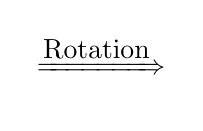
\begin{tikzpicture}
    \draw (0,0) node (arrow) 
{$\xRightarrow{\text{\normalsize Rotation}}$};
    \end{tikzpicture} 
     &
      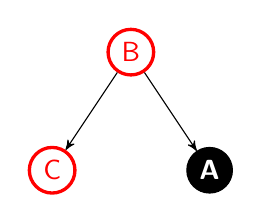
\begin{tikzpicture}[->,>=stealth',level/.style={sibling distance = 2cm,
  level distance = 1.5cm}] 
\node [arn_r] (g) {B}
child  {
	node [arn_r] {C}
}
child{
	node [arn_n] {A}
} 
;
\end{tikzpicture}
    &
	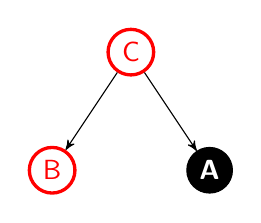
\begin{tikzpicture}[->,>=stealth',level/.style={sibling distance = 2cm,
	  level distance = 1.5cm}] 
	\node [arn_r] (g) {C}
	child  {
		node [arn_r] {B}
	}
	child{
		node [arn_n] {A}
	} 
	;
	\end{tikzpicture}
     \\ 
     \\
     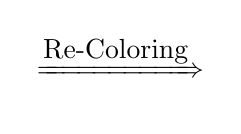
\begin{tikzpicture}
    \draw (0,0) node (arrow) 
{$\xRightarrow{\text{\normalsize Re-Coloring}}$};
    \end{tikzpicture} 
     &
      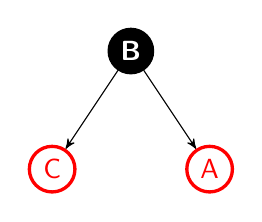
\begin{tikzpicture}[->,>=stealth',level/.style={sibling distance = 2cm,
  level distance = 1.5cm}] 
\node [arn_n] (g) {B}
child  {
	node [arn_r] {C}
}
child{
	node [arn_r] {A}
} 
;
\end{tikzpicture}
    &
	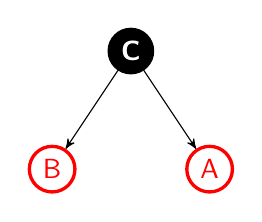
\begin{tikzpicture}[->,>=stealth',level/.style={sibling distance = 2cm,
	  level distance = 1.5cm}] 
	\node [arn_n] (g) {C}
	child  {
		node [arn_r] {B}
	}
	child{
		node [arn_r] {A}
	} 
	;
	\end{tikzpicture}
  \end{tabular}
  \egroup
\end{center}
\end{latin}



حالا که مفاهیم و نکات جدیدی در ارتباط با درخت قرمز-مشکی یاد گرفتیم می توانیم به ساخت درخت قبلی خودمان ادامه دهیم :


حال می دانیم در برخورد قرمز ها در این نمونه چون
\lr{Uncle}
مشکی است ، از چرخش و سپس  در صورت  تغییر رنگ نیاز از تغییر رنگ استفاده می کنیم :





\begin{latin}
\begin{center}
  \bgroup
  \def\arraystretch{1.5}%
  \begin{tabular}{ D C  }
    \begin{tikzpicture}
    \draw (0,0) node (arrow) 
{$\Longrightarrow{\text{\normalsize}}$};
    \end{tikzpicture} 
    &
    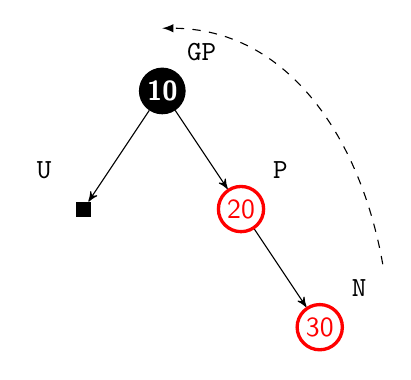
\begin{tikzpicture}[->,>=stealth',level/.style={sibling distance = 2cm,
  level distance = 1.5cm}] 
\node [arn_n] (g) {10}
child  {
	node [arn_x] (u) {}
}
child{
	node [arn_r] (p) {20}
	child [missing] {}
	child{
		node [arn_r] (n) {30}
	} 
};
\node at (g) [xshift=0.5cm,yshift=0.5cm] {\normalsize\ttfamily GP};
\node at (p) [xshift=0.5cm,yshift=0.5cm] {\normalsize\ttfamily P};
\node at (u) [xshift=-0.5cm,yshift=0.5cm] {\normalsize\ttfamily U};
\node at (n) [xshift=0.5cm,yshift=0.5cm] {\normalsize\ttfamily N};

\coordinate (A) at ([yshift=.8cm,xshift=0.8cm]n);
%\coordinate (C) at ([yshift=.5cm,xshift=1cm]r);
\coordinate (C) at ([yshift=.5cm]g.north);

%\draw[dashed] plot[smooth] coordinates {(C) (A)};
\draw[->,>=latex,dashed] (A) to[out=100,in=0] (C);
\end{tikzpicture}
     \\ 
  \end{tabular}
  \egroup
\end{center}
\end{latin}




\begin{latin}
\begin{center}
  \bgroup
  \def\arraystretch{1.5}%
  \begin{tabular}{ D C D C  }
     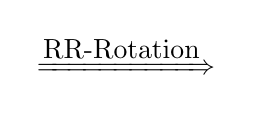
\begin{tikzpicture}
    \draw (0,0) node (arrow) 
{$\xRightarrow{\text{\normalsize RR-Rotation}}$};
    \end{tikzpicture} 
     &
      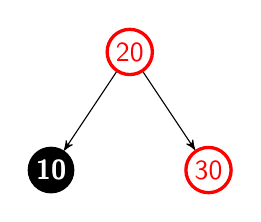
\begin{tikzpicture}[->,>=stealth',level/.style={sibling distance = 2cm,
  level distance = 1.5cm}] 
\node [arn_r] (g) {20}
child  {
	node [arn_n] {10}
}
child{
	node [arn_r] {30}
} 
;
\end{tikzpicture}
&
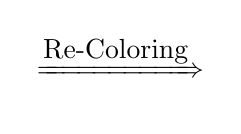
\begin{tikzpicture}
    \draw (0,0) node (arrow) 
{$\xRightarrow{\text{\normalsize Re-Coloring}}$};
    \end{tikzpicture} 
    &
    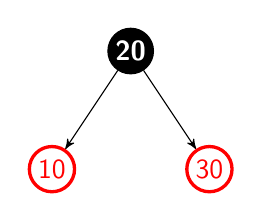
\begin{tikzpicture}[->,>=stealth',level/.style={sibling distance = 2cm,
  level distance = 1.5cm}] 
\node [arn_n] (g) {20}
child  {
	node [arn_r] {10}
}
child{
	node [arn_r] {30}
} 
;
\end{tikzpicture}
     \\ 
  \end{tabular}
  \egroup
\end{center}
\end{latin}






سپس عنصر 
\tikz \node [arn_r]  {50} ;
را اضافه می کنیم ، به خاطر اینکه این عنصر تازه وارد است به رنگ قرمز می باشد ، درج این عنصر مشکل 
\textbf{
برخورد قرمزها  
}
را به وجود می آورد ، از آنجایی که 
\lr{Uncle}
به رنگ قرمز است از روش تغییر رنگ استفاده می کنیم .






\begin{latin}
\begin{center}
  \bgroup
  \def\arraystretch{1.5}%
  \begin{tabular}{ D C D C  }
     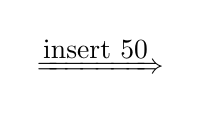
\begin{tikzpicture}
    \draw (0,0) node (arrow) 
{$\xRightarrow{\text{\normalsize insert 50}}$};
    \end{tikzpicture} 
     &
      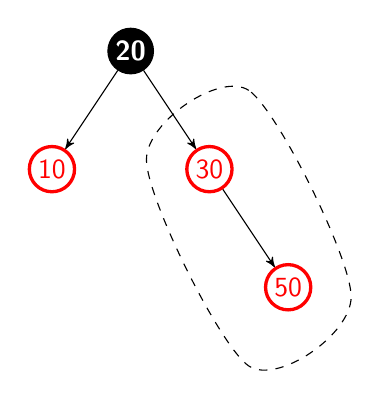
\begin{tikzpicture}[->,>=stealth',level/.style={sibling distance = 2cm,
  level distance = 1.5cm}] 
\node [arn_n] (g) {20}
child  {
	node [arn_r] (u) {10}
}
child{
	node [arn_r] (p) {30}
	child [missing] {}
	child{
	    node [arn_r] (n) {50}
    } 
};
%\node at (g) [xshift=0.5cm,yshift=0.5cm] {\normalsize\ttfamily GP};
%\node at (p) [xshift=0.5cm,yshift=0.5cm] {\normalsize\ttfamily P};
%\node at (u) [xshift=-0.5cm,yshift=0.5cm] {\normalsize\ttfamily U};
%\node at (n) [xshift=0.5cm,yshift=0.5cm] {\normalsize\ttfamily N};

\coordinate (A) at ([yshift=-0.12cm,xshift=0.8cm]n);
\coordinate (AA) at ([yshift=-1cm,xshift=-0.5cm]n);
%\coordinate (C) at ([yshift=.5cm,xshift=1cm]r);
\coordinate (C) at ([yshift=.5cm]g.north);

\coordinate (B) at ([yshift=1cm,xshift=0.5cm]p);
\coordinate (BB) at ([yshift=0.12cm,xshift=-0.8cm]p);

\draw[dashed] plot[smooth cycle] coordinates {(A) (B) (BB)  (AA)};
%\draw[->,>=latex,dashed] (A) to[out=100,in=0] (C);
\end{tikzpicture}
     \\ 
  \end{tabular}
  \egroup
\end{center}
\end{latin}








\begin{latin}
\begin{center}
  \bgroup
  \def\arraystretch{1.5}%
  \begin{tabular}{ D C D C  }
     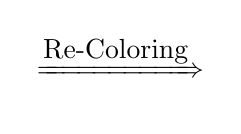
\begin{tikzpicture}
    \draw (0,0) node (arrow) 
{$\xRightarrow{\text{\normalsize Re-Coloring}}$};
    \end{tikzpicture} 
     &
      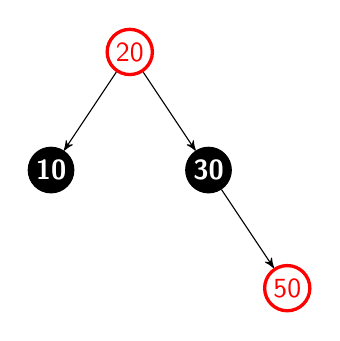
\begin{tikzpicture}[->,>=stealth',level/.style={sibling distance = 2cm,
  level distance = 1.5cm}] 
\node [arn_r] (g) {20}
child  {
	node [arn_n] (u) {10}
}
child{
	node [arn_n] (p) {30}
	child [missing] {}
	child{
	    node [arn_r] (n) {50}
    } 
};
%\node at (g) [xshift=0.5cm,yshift=0.5cm] {\normalsize\ttfamily GP};
%\node at (p) [xshift=0.5cm,yshift=0.5cm] {\normalsize\ttfamily P};
%\node at (u) [xshift=-0.5cm,yshift=0.5cm] {\normalsize\ttfamily U};
%\node at (n) [xshift=0.5cm,yshift=0.5cm] {\normalsize\ttfamily N};

%\coordinate (A) at ([yshift=-0.12cm,xshift=0.8cm]n);
%\coordinate (AA) at ([yshift=-1cm,xshift=-0.5cm]n);
%\coordinate (C) at ([yshift=.5cm,xshift=1cm]r);
%\coordinate (C) at ([yshift=.5cm]g.north);

%\coordinate (B) at ([yshift=1cm,xshift=0.5cm]p);
%\coordinate (BB) at ([yshift=0.12cm,xshift=-0.8cm]p);

%\draw[dashed] plot[smooth cycle] coordinates {(A) (B) (BB)  (AA)};
%\draw[->,>=latex,dashed] (A) to[out=100,in=0] (C);
\end{tikzpicture}
     \\ 
  \end{tabular}
  \egroup
\end{center}
\end{latin}



چون بعد از تغییر رنگ ، نود
\lr{(Grand Parent)}
همان ریشه ی درخت بود آن را به رنگ مشکی تغییر می دهیم .




\begin{latin}
\begin{center}
\begin{lstlisting}[language=C++]
if ( GP == root ) {
	Re-Color GP to Black
}
\end{lstlisting}
\end{center}
\end{latin}







\begin{latin}
\begin{center}
  \bgroup
  \def\arraystretch{1.5}%
  \begin{tabular}{ C C  }
     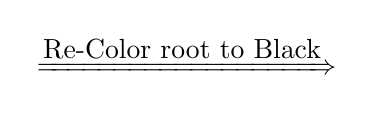
\begin{tikzpicture}
    \draw (0,0) node (arrow) 
{$\xRightarrow{\text{\normalsize Re-Color root to Black}}$};
    \end{tikzpicture} 
     &
      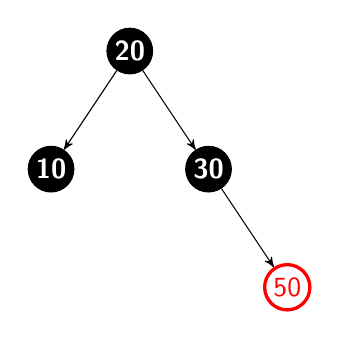
\begin{tikzpicture}[->,>=stealth',level/.style={sibling distance = 2cm,
  level distance = 1.5cm}] 
\node [arn_n] (g) {20}
child  {
	node [arn_n] (u) {10}
}
child{
	node [arn_n] (p) {30}
	child [missing] {}
	child{
	    node [arn_r] (n) {50}
    } 
};
%\node at (g) [xshift=0.5cm,yshift=0.5cm] {\normalsize\ttfamily GP};
%\node at (p) [xshift=0.5cm,yshift=0.5cm] {\normalsize\ttfamily P};
%\node at (u) [xshift=-0.5cm,yshift=0.5cm] {\normalsize\ttfamily U};
%\node at (n) [xshift=0.5cm,yshift=0.5cm] {\normalsize\ttfamily N};

%\coordinate (A) at ([yshift=-0.12cm,xshift=0.8cm]n);
%\coordinate (AA) at ([yshift=-1cm,xshift=-0.5cm]n);
%\coordinate (C) at ([yshift=.5cm,xshift=1cm]r);
%\coordinate (C) at ([yshift=.5cm]g.north);

%\coordinate (B) at ([yshift=1cm,xshift=0.5cm]p);
%\coordinate (BB) at ([yshift=0.12cm,xshift=-0.8cm]p);

%\draw[dashed] plot[smooth cycle] coordinates {(A) (B) (BB)  (AA)};
%\draw[->,>=latex,dashed] (A) to[out=100,in=0] (C);
\end{tikzpicture}
     \\ 
  \end{tabular}
  \egroup
\end{center}
\end{latin}





سپس عنصر 
\tikz \node [arn_r]  {40} ;
را اضافه می کنیم ، به خاطر اینکه این عنصر تازه وارد است به رنگ قرمز می باشد ، درج این عنصر مشکل 
\textbf{
برخورد قرمزها  
}
را به وجود می آورد ، از آنجایی که 
\lr{Uncle}
به رنگ مشکی است از روش چرخش استفاده می کنیم .






\begin{latin}
\begin{center}
  \bgroup
  \def\arraystretch{1.5}%
  \begin{tabular}{ C C  }
     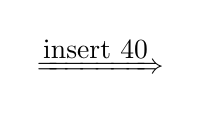
\begin{tikzpicture}
    \draw (0,0) node (arrow) 
{$\xRightarrow{\text{\normalsize insert 40}}$};
    \end{tikzpicture} 
     &
      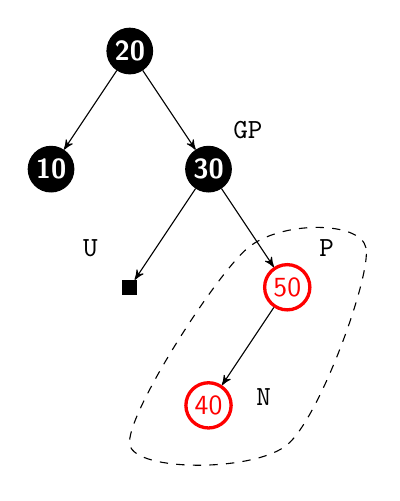
\begin{tikzpicture}[->,>=stealth',level/.style={sibling distance = 2cm,
  level distance = 1.5cm}] 
\node [arn_n]  {20}
child  {
	node [arn_n]  {10}
}
child{
	node [arn_n] (g) {30}
	child {
	    node [arn_x] (u) {}
	}
	child{
	    node [arn_r] (p) {50}
	    child{
	       node [arn_r] (n) {40}
	    } child [missing] {}
    } 
};
\node at (g) [xshift=0.5cm,yshift=0.5cm] {\normalsize\ttfamily GP};
\node at (p) [xshift=0.5cm,yshift=0.5cm] {\normalsize\ttfamily P};
\node at (u) [xshift=-0.5cm,yshift=0.5cm] {\normalsize\ttfamily U};
\node at (n) [xshift=0.7cm,yshift=0.1cm] {\normalsize\ttfamily N};

\coordinate (A) at ([yshift=-0.5cm,xshift=1cm]n);
\coordinate (AA) at ([yshift=-0.5cm,xshift=-1cm]n);
%\coordinate (C) at ([yshift=.5cm,xshift=1cm]r);
%\coordinate (C) at ([yshift=.5cm]g.north);

\coordinate (B) at ([yshift=0.5cm,xshift=1cm]p);
\coordinate (BB) at ([yshift=0.5cm,xshift=-0.5cm]p);

\draw[dashed] plot[smooth cycle] coordinates {(A) (B) (BB)  (AA)};
%\draw[->,>=latex,dashed] (A) to[out=100,in=0] (C);
\end{tikzpicture}
     \\ 
  \end{tabular}
  \egroup
\end{center}
\end{latin}






\begin{latin}
\begin{center}
  \bgroup
  \def\arraystretch{1.5}%
  \begin{tabular}{ C C  }
     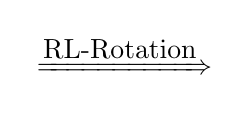
\begin{tikzpicture}
    \draw (0,0) node (arrow) 
{$\xRightarrow{\text{\normalsize RL-Rotation}}$};
    \end{tikzpicture} 
     &
      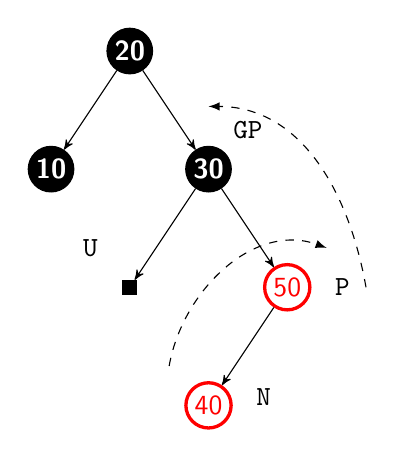
\begin{tikzpicture}[->,>=stealth',level/.style={sibling distance = 2cm,
  level distance = 1.5cm}] 
\node [arn_n]  {20}
child  {
	node [arn_n]  {10}
}
child{
	node [arn_n] (g) {30}
	child {
	    node [arn_x] (u) {}
	}
	child{
	    node [arn_r] (p) {50}
	    child{
	       node [arn_r] (n) {40}
	    } child [missing] {}
    } 
};
\node at (g) [xshift=0.5cm,yshift=0.5cm] {\normalsize\ttfamily GP};
\node at (p) [xshift=0.7cm,yshift=0cm] {\normalsize\ttfamily P};
\node at (u) [xshift=-0.5cm,yshift=0.5cm] {\normalsize\ttfamily U};
\node at (n) [xshift=0.7cm,yshift=0.1cm] {\normalsize\ttfamily N};

%\coordinate (A) at ([yshift=-0.5cm,xshift=1cm]n);
%\coordinate (AA) at ([yshift=-0.5cm,xshift=-1cm]n);
%\coordinate (C) at ([yshift=.5cm,xshift=1cm]r);
%\coordinate (C) at ([yshift=.5cm]g.north);

%\coordinate (B) at ([yshift=0.5cm,xshift=1cm]p);
%\coordinate (BB) at ([yshift=0.5cm,xshift=-0.5cm]p);

%\draw[dashed] plot[smooth cycle] coordinates {(A) (B) (BB)  (AA)};
%\draw[->,>=latex,dashed] (A) to[out=100,in=0] (C);
\coordinate (A) at ([xshift=1cm]p);
\coordinate (C) at ([yshift=.5cm]g.north);

\coordinate (E) at ([yshift=0.5cm,xshift=-0.5cm]n);
%\coordinate (F) at ([yshift=.5cm]a);
\coordinate (G) at ([xshift=0.5cm,yshift=0.5cm]p);

%\draw[dashed] plot[smooth] coordinates {(C) (A)};
\draw[->,>=latex,dashed] (A) to[out=100,in=0] (C);
\draw[->,>=latex,dashed] (E) to[out=80,in=160] (G) ;
\end{tikzpicture}
     \\ 
  \end{tabular}
  \egroup
\end{center}
\end{latin}







\begin{latin}
\begin{center}
  \bgroup
  \def\arraystretch{1.5}%
  \begin{tabular}{ C C  }
     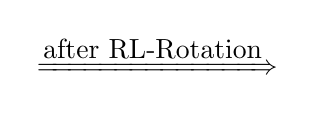
\begin{tikzpicture}
    \draw (0,0) node (arrow) 
{$\xRightarrow{\text{\normalsize after RL-Rotation}}$};
    \end{tikzpicture} 
     &
      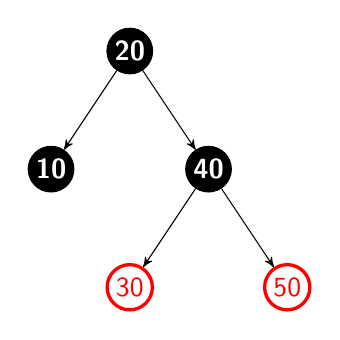
\begin{tikzpicture}[->,>=stealth',level/.style={sibling distance = 2cm,
  level distance = 1.5cm}] 
\node [arn_n] (g) {20}
child  {
	node [arn_n]  {10}
}
child{
    node [arn_n]  {40}
	child {
	    node [arn_r]  {30}
	}
	child{
	    node [arn_r]  {50}
    } 
};
%\node at (g) [xshift=0.5cm,yshift=0.5cm] {\normalsize\ttfamily GP};
%\node at (p) [xshift=0.7cm,yshift=0cm] {\normalsize\ttfamily P};
%\node at (u) [xshift=-0.5cm,yshift=0.5cm] {\normalsize\ttfamily U};
%\node at (n) [xshift=0.7cm,yshift=0.1cm] {\normalsize\ttfamily N};

%\coordinate (A) at ([yshift=-0.5cm,xshift=1cm]n);
%\coordinate (AA) at ([yshift=-0.5cm,xshift=-1cm]n);
%\coordinate (C) at ([yshift=.5cm,xshift=1cm]r);
%\coordinate (C) at ([yshift=.5cm]g.north);

%\coordinate (B) at ([yshift=0.5cm,xshift=1cm]p);
%\coordinate (BB) at ([yshift=0.5cm,xshift=-0.5cm]p);

%\draw[dashed] plot[smooth cycle] coordinates {(A) (B) (BB)  (AA)};
%\draw[->,>=latex,dashed] (A) to[out=100,in=0] (C);
\end{tikzpicture}
     \\ 
  \end{tabular}
  \egroup
\end{center}
\end{latin}






سپس عنصر 
\tikz \node [arn_r]  {60} ;
را اضافه می کنیم ، به خاطر اینکه این عنصر تازه وارد است به رنگ قرمز می باشد ، درج این عنصر مشکل 
\textbf{
برخورد قرمزها  
}
را به وجود می آورد ، از آنجایی که 
\lr{Uncle}
به رنگ قرمز است از روش تغییر رنگ استفاده می کنیم .







\begin{latin}
\begin{center}
  \bgroup
  \def\arraystretch{1.5}%
  \begin{tabular}{ C C  }
     \begin{tikzpicture}
    \draw (0,0) node (arrow) 
{$\xRightarrow{\text{\normalsize insert 60}}$};
    \end{tikzpicture} 
     &
      \begin{tikzpicture}[->,>=stealth',level/.style={sibling distance = 2cm,
  level distance = 1.5cm}] 
\node [arn_n] {20}
child  {
	node [arn_n]  {10}
}
child{
    node [arn_n] (g) {40}
	child {
	    node [arn_r] (u) {30}
	}
	child{
	    node [arn_r] (p) {50}
	    child [missing] {}
	    child {
	        node [arn_r] (n) {60}
	    }
    } 
};
\node at (g) [xshift=0.5cm,yshift=0.5cm] {\normalsize\ttfamily GP};
\node at (p) [xshift=0.7cm,yshift=0cm] {\normalsize\ttfamily P};
\node at (u) [xshift=-0.5cm,yshift=0.5cm] {\normalsize\ttfamily U};
\node at (n) [xshift=0.6cm,yshift=0.1cm] {\normalsize\ttfamily N};

\coordinate (A) at ([yshift=-0.12cm,xshift=0.8cm]n);
\coordinate (AA) at ([yshift=-1cm,xshift=-0.5cm]n);
%\coordinate (C) at ([yshift=.5cm,xshift=1cm]r);
\coordinate (C) at ([yshift=.5cm]g.north);

\coordinate (B) at ([yshift=1cm,xshift=0.5cm]p);
\coordinate (BB) at ([yshift=0.12cm,xshift=-0.8cm]p);

\draw[dashed] plot[smooth cycle] coordinates {(A) (B) (BB)  (AA)};
%\draw[->,>=latex,dashed] (A) to[out=100,in=0] (C);
\end{tikzpicture}
     \\ 
  \end{tabular}
  \egroup
\end{center}
\end{latin}








\begin{latin}
\begin{center}
  \bgroup
  \def\arraystretch{1.5}%
  \begin{tabular}{ C C  }
     \begin{tikzpicture}
    \draw (0,0) node (arrow) 
{$\xRightarrow{\text{\normalsize Re-Coloring}}$};
    \end{tikzpicture} 
     &
      \begin{tikzpicture}[->,>=stealth',level/.style={sibling distance = 2cm,
  level distance = 1.5cm}] 
\node [arn_n]  {20}
child  {
	node [arn_n] {10}
}
child{
    node [arn_r] (g) {40}
	child {
	    node [arn_n] (u) {30}
	}
	child{
	    node [arn_n] (p) {50}
	    child [missing] {}
	    child {
	        node [arn_r] (n) {60}
	    }
    } 
};
\node at (g) [xshift=0.5cm,yshift=0.5cm] {\normalsize\ttfamily GP};
\node at (p) [xshift=0.7cm,yshift=0cm] {\normalsize\ttfamily P};
\node at (u) [xshift=-0.5cm,yshift=0.5cm] {\normalsize\ttfamily U};
\node at (n) [xshift=0.6cm,yshift=0.1cm] {\normalsize\ttfamily N};

%\coordinate (A) at ([yshift=-0.12cm,xshift=0.8cm]n);
%\coordinate (AA) at ([yshift=-1cm,xshift=-0.5cm]n);
%\coordinate (C) at ([yshift=.5cm,xshift=1cm]r);
%\coordinate (C) at ([yshift=.5cm]g.north);

%\coordinate (B) at ([yshift=1cm,xshift=0.5cm]p);
%\coordinate (BB) at ([yshift=0.12cm,xshift=-0.8cm]p);

%\draw[dashed] plot[smooth cycle] coordinates {(A) (B) (BB)  (AA)};
%\draw[->,>=latex,dashed] (A) to[out=100,in=0] (C);
\end{tikzpicture}
     \\ 
  \end{tabular}
  \egroup
\end{center}
\end{latin}





\begin{tcolorbox}

حال برای نود
\lr{Grand Parent}
چک می کنیم که بعد از تغییر رنگ مشکل برخورد قرمزها به وجود آمده است یا خیر و این کار را تا زمانی که ببینیم برخورد قرمز وجود ندارد ادامه می دهیم .

\noindent
در این نمونه 
\lr{Grand Parent}
مشکی می باشد و بنابراین برخورد قرمزها به وجود نمی آید .
\end{tcolorbox}






سپس عنصر 
\tikz \node [arn_r]  {70} ;
را اضافه می کنیم ، به خاطر اینکه این عنصر تازه وارد است به رنگ قرمز می باشد ، درج این عنصر مشکل 
\textbf{
برخورد قرمزها  
}
را به وجود می آورد ، از آنجایی که 
\lr{Uncle}
به رنگ مشکی است از روش چرخش استفاده می کنیم .




\begin{latin}
\begin{center}
  \bgroup
  \def\arraystretch{1.5}%
  \begin{tabular}{ C C  }
     \begin{tikzpicture}
    \draw (0,0) node (arrow) 
{$\xRightarrow{\text{\normalsize insert 70}}$};
    \end{tikzpicture} 
     &
      \begin{tikzpicture}[->,>=stealth',level/.style={sibling distance = 2cm,
  level distance = 1.5cm}] 
\node [arn_n]  {20}
child  {
	node [arn_n] {10}
}
child{
    node [arn_r]  {40}
	child {
	    node [arn_n]  {30}
	}
	child{
	    node [arn_n] (g) {50}
	    child  {
	         node [arn_x] (u) {}
	    }
	    child {
	        node [arn_r] (p) {60}
	        child [missing] {}
	        child {
	             node [arn_r] (n) {70}
	        }
	    }
    } 
};
\node at (g) [xshift=0.5cm,yshift=0.5cm] {\normalsize\ttfamily GP};
\node at (p) [xshift=0.7cm,yshift=0cm] {\normalsize\ttfamily P};
\node at (u) [xshift=-0.5cm,yshift=0.5cm] {\normalsize\ttfamily U};
\node at (n) [xshift=0.6cm,yshift=0.1cm] {\normalsize\ttfamily N};

\coordinate (A) at ([yshift=-0.12cm,xshift=0.8cm]n);
\coordinate (AA) at ([yshift=-1cm,xshift=-0.5cm]n);
%\coordinate (C) at ([yshift=.5cm,xshift=1cm]r);
%\coordinate (C) at ([yshift=.5cm]g.north);

\coordinate (B) at ([yshift=1cm,xshift=0.5cm]p);
\coordinate (BB) at ([yshift=0.12cm,xshift=-0.8cm]p);

\draw[dashed] plot[smooth cycle] coordinates {(A) (B) (BB)  (AA)};
%\draw[->,>=latex,dashed] (A) to[out=100,in=0] (C);
\end{tikzpicture}
     \\ 
  \end{tabular}
  \egroup
\end{center}
\end{latin}








\begin{latin}
\begin{center}
  \bgroup
  \def\arraystretch{1.5}%
  \begin{tabular}{ C C  }
     \begin{tikzpicture}
    \draw (0,0) node (arrow) 
{$\xRightarrow{\text{\normalsize RR-Rotation}}$};
    \end{tikzpicture} 
     &
      \begin{tikzpicture}[->,>=stealth',level/.style={sibling distance = 2cm,
  level distance = 1.5cm}] 
\node [arn_n]  {20}
child  {
	node [arn_n] {10}
}
child{
    node [arn_r]  {40}
	child {
	    node [arn_n]  {30}
	}
	child{
	    node [arn_n] (g) {50}
	    child  {
	         node [arn_x] (u) {}
	    }
	    child {
	        node [arn_r] (p) {60}
	        child [missing] {}
	        child {
	             node [arn_r] (n) {70}
	        }
	    }
    } 
};
\node at (g) [xshift=0.5cm,yshift=0.5cm] {\normalsize\ttfamily GP};
\node at (p) [xshift=0.7cm,yshift=0cm] {\normalsize\ttfamily P};
\node at (u) [xshift=-0.5cm,yshift=0.5cm] {\normalsize\ttfamily U};
\node at (n) [xshift=0.6cm,yshift=0.1cm] {\normalsize\ttfamily N};

%\coordinate (A) at ([yshift=-0.12cm,xshift=0.8cm]n);
%\coordinate (AA) at ([yshift=-1cm,xshift=-0.5cm]n);
%\coordinate (C) at ([yshift=.5cm,xshift=1cm]r);
%\coordinate (C) at ([yshift=.5cm]g.north);

%\coordinate (B) at ([yshift=1cm,xshift=0.5cm]p);
%\coordinate (BB) at ([yshift=0.12cm,xshift=-0.8cm]p);

%\draw[dashed] plot[smooth cycle] coordinates {(A) (B) (BB)  (AA)};
%\draw[->,>=latex,dashed] (A) to[out=100,in=0] (C);
\coordinate (A) at ([yshift=.8cm,xshift=0.8cm]n);
%\coordinate (C) at ([yshift=.5cm,xshift=1cm]r);
\coordinate (C) at ([yshift=.5cm]g.north);

%\draw[dashed] plot[smooth] coordinates {(C) (A)};
\draw[->,>=latex,dashed] (A) to[out=100,in=0] (C);
\end{tikzpicture}
     \\ 
  \end{tabular}
  \egroup
\end{center}
\end{latin}







\begin{latin}
\begin{center}
  \bgroup
  \def\arraystretch{1.5}%
  \begin{tabular}{ C C  }
     \begin{tikzpicture}
    \draw (0,0) node (arrow) 
{$\xRightarrow{\text{\normalsize after RR-Rotation}}$};
    \end{tikzpicture} 
     &
      \begin{tikzpicture}[->,>=stealth',level/.style={sibling distance = 2cm,
  level distance = 1.5cm}] 
\node [arn_n]  {20}
child  {
	node [arn_n] {10}
}
child{
    node [arn_r]  {40}
	child {
	    node [arn_n]  {30}
	}
	child{
	     node [arn_n] (p) {60}
	        child {
	             node [arn_r] (g) {50}
	        }
	        child {
	             node [arn_r] (n) {70}
	        }
    } 
};
%\node at (g) [xshift=0.5cm,yshift=0.5cm] {\normalsize\ttfamily GP};
%\node at (p) [xshift=0.7cm,yshift=0cm] {\normalsize\ttfamily P};
%\node at (u) [xshift=-0.5cm,yshift=0.5cm] {\normalsize\ttfamily U};
%\node at (n) [xshift=0.6cm,yshift=0.1cm] {\normalsize\ttfamily N};

%\coordinate (A) at ([yshift=-0.12cm,xshift=0.8cm]n);
%\coordinate (AA) at ([yshift=-1cm,xshift=-0.5cm]n);
%\coordinate (C) at ([yshift=.5cm,xshift=1cm]r);
%\coordinate (C) at ([yshift=.5cm]g.north);

%\coordinate (B) at ([yshift=1cm,xshift=0.5cm]p);
%\coordinate (BB) at ([yshift=0.12cm,xshift=-0.8cm]p);

%\draw[dashed] plot[smooth cycle] coordinates {(A) (B) (BB)  (AA)};
%\draw[->,>=latex,dashed] (A) to[out=100,in=0] (C);
\end{tikzpicture}
     \\ 
  \end{tabular}
  \egroup
\end{center}
\end{latin}






سپس عنصر 
\tikz \node [arn_r]  {80} ;
را اضافه می کنیم ، به خاطر اینکه این عنصر تازه وارد است به رنگ قرمز می باشد ، درج این عنصر مشکل 
\textbf{
برخورد قرمزها  
}
را به وجود می آورد ، از آنجایی که 
\lr{Uncle}
به رنگ قرمز است از روش تغییر رنگ استفاده می کنیم .






\begin{latin}
\begin{center}
  \bgroup
  \def\arraystretch{1.5}%
  \begin{tabular}{ C C  }
     \begin{tikzpicture}
    \draw (0,0) node (arrow) 
{$\xRightarrow{\text{\normalsize insert 80}}$};
    \end{tikzpicture} 
     &
      \begin{tikzpicture}[->,>=stealth',level/.style={sibling distance = 2cm,
  level distance = 1.5cm}] 
\node [arn_n]  {20}
child  {
	node [arn_n] {10}
}
child{
    node [arn_r]  {40}
	child {
	    node [arn_n]  {30}
	}
	child{
	     node [arn_n] (g) {60}
	        child {
	             node [arn_r] (u) {50}
	        }
	        child {
	             node [arn_r] (p) {70}
	             child [missing] {}
	             child {
	                 node [arn_r] (n) {80}
	             }
	        }
    } 
};
\node at (g) [xshift=0.5cm,yshift=0.5cm] {\normalsize\ttfamily GP};
\node at (p) [xshift=0.7cm,yshift=0cm] {\normalsize\ttfamily P};
\node at (u) [xshift=-0.5cm,yshift=0.5cm] {\normalsize\ttfamily U};
\node at (n) [xshift=0.6cm,yshift=0.1cm] {\normalsize\ttfamily N};

\coordinate (A) at ([yshift=-0.12cm,xshift=0.8cm]n);
\coordinate (AA) at ([yshift=-1cm,xshift=-0.5cm]n);
%\coordinate (C) at ([yshift=.5cm,xshift=1cm]r);
%\coordinate (C) at ([yshift=.5cm]g.north);

\coordinate (B) at ([yshift=1cm,xshift=0.5cm]p);
\coordinate (BB) at ([yshift=0.12cm,xshift=-0.8cm]p);

\draw[dashed] plot[smooth cycle] coordinates {(A) (B) (BB)  (AA)};
%\draw[->,>=latex,dashed] (A) to[out=100,in=0] (C);
\end{tikzpicture}
     \\ 
  \end{tabular}
  \egroup
\end{center}
\end{latin}











\begin{latin}
\begin{center}
  \bgroup
  \def\arraystretch{1.5}%
  \begin{tabular}{ C C  }
     \begin{tikzpicture}
    \draw (0,0) node (arrow) 
{$\xRightarrow{\text{\normalsize Re-Coloring}}$};
    \end{tikzpicture} 
     &
      \begin{tikzpicture}[->,>=stealth',level/.style={sibling distance = 2cm,
  level distance = 1.5cm}]
\node [arn_n]  {20}
child  {
	node [arn_n] {10}
}
child{
    node [arn_r] (gp) {40}
	child {
	    node [arn_n]  {30}
	}
	child{
	     node [arn_r] (g) {60}
	        child {
	             node [arn_n] (u) {50}
	        }
	        child {
	             node [arn_n] (p) {70}
	             child [missing] {}
	             child {
	                 node [arn_r] (n) {80}
	             }
	        }
    } 
};
\node at (g) [xshift=0.5cm,yshift=0.5cm] {\normalsize\ttfamily GP};
\node at (p) [xshift=0.7cm,yshift=0cm] {\normalsize\ttfamily P};
\node at (u) [xshift=-0.5cm,yshift=0.5cm] {\normalsize\ttfamily U};
\node at (n) [xshift=0.6cm,yshift=0.1cm] {\normalsize\ttfamily N};

\coordinate (A) at ([yshift=-0.12cm,xshift=0.8cm]g);
\coordinate (AA) at ([yshift=-1cm,xshift=-0.5cm]g);
%\coordinate (C) at ([yshift=.5cm,xshift=1cm]r);
%\coordinate (C) at ([yshift=.5cm]g.north);

\coordinate (B) at ([yshift=1cm,xshift=0.5cm]gp);
\coordinate (BB) at ([yshift=0.12cm,xshift=-0.8cm]gp);

\draw[dashed] plot[smooth cycle] coordinates {(A) (B) (BB)  (AA)};
%\draw[->,>=latex,dashed] (A) to[out=100,in=0] (C);
\end{tikzpicture}
     \\ 
  \end{tabular}
  \egroup
\end{center}
\end{latin}








\begin{tcolorbox}

حال برای نود
\lr{Grand Parent}
چک می کنیم که بعد از تغییر رنگ مشکل برخورد قرمزها به وجود آمده است یا خیر و این کار را تا زمانی که ببینیم برخورد قرمز وجود ندارد ادامه می دهیم .

\noindent
در این نمونه 
\lr{Grand Parent}
قرمز می باشد و بنابراین برخورد قرمزها به وجود می آید ، از آنجایی که 
\lr{Uncle}
جدید به رنگ مشکی است از روش چرخش استفاده می کنیم .
\end{tcolorbox}















\begin{latin}
\begin{center}
  \bgroup
  \def\arraystretch{1.5}%
  \begin{tabular}{ C C  }
     \begin{tikzpicture}
    \draw (0,0) node (arrow) 
{$\xRightarrow{\text{\normalsize Re-Coloring}}$};
    \end{tikzpicture} 
     &
      \begin{tikzpicture}[->,>=stealth',level/.style={sibling distance = 2cm,
  level distance = 1.5cm}]
\node [arn_n] (g) {20}
child  {
	node [arn_n] (u) {10}
}
child{
    node [arn_r] (p) {40}
	child {
	    node [arn_n]  {30}
	}
	child{
	     node [arn_r] (n) {60}
	        child {
	             node [arn_n] {50}
	        }
	        child {
	             node [arn_n] {70}
	             child [missing] {}
	             child {
	                 node [arn_r] {80}
	             }
	        }
    } 
};
\node at (g) [xshift=0.5cm,yshift=0.5cm] {\normalsize\ttfamily GP};
\node at (p) [xshift=0.7cm,yshift=0cm] {\normalsize\ttfamily P};
\node at (u) [xshift=-0.5cm,yshift=0.5cm] {\normalsize\ttfamily U};
\node at (n) [xshift=0.6cm,yshift=0.1cm] {\normalsize\ttfamily N};

%\coordinate (A) at ([yshift=-0.12cm,xshift=0.8cm]g);
%\coordinate (AA) at ([yshift=-1cm,xshift=-0.5cm]g);
%\coordinate (C) at ([yshift=.5cm,xshift=1cm]r);
%\coordinate (C) at ([yshift=.5cm]g.north);

%\coordinate (B) at ([yshift=1cm,xshift=0.5cm]gp);
%\coordinate (BB) at ([yshift=0.12cm,xshift=-0.8cm]gp);

%\draw[dashed] plot[smooth cycle] coordinates {(A) (B) (BB)  (AA)};
%\draw[->,>=latex,dashed] (A) to[out=100,in=0] (C);
\coordinate (A) at ([yshift=.8cm,xshift=0.8cm]n);
%\coordinate (C) at ([yshift=.5cm,xshift=1cm]r);
\coordinate (C) at ([yshift=.5cm]g.north);

%\draw[dashed] plot[smooth] coordinates {(C) (A)};
\draw[->,>=latex,dashed] (A) to[out=100,in=0] (C);
\end{tikzpicture}
     \\ 
  \end{tabular}
  \egroup
\end{center}
\end{latin}








\begin{latin}
\begin{center}
  \bgroup
  \def\arraystretch{1.5}%
  \begin{tabular}{ C C  }
     \begin{tikzpicture}
    \draw (0,0) node (arrow) 
{$\xRightarrow{\text{\normalsize RR-Rotation}}$};
    \end{tikzpicture} 
     &
      \begin{tikzpicture}[->,>=stealth',level/.style={sibling distance = 4cm/#1,
  level distance = 1.5cm}]
\node [arn_n]  {40}
child  {
     node [arn_r] {20}
	child {
		node [arn_n] {10}
	}
	child {
	    node [arn_n]  {30}
	}
}
child{
	     node [arn_r] {60}
	        child {
	             node [arn_n] {50}
	        }
	        child {
	             node [arn_n] {70}
	             child [missing] {}
	             child {
	                 node [arn_r] {80}
	             }
	        }
};
%\node at (g) [xshift=0.5cm,yshift=0.5cm] {\normalsize\ttfamily GP};
%\node at (p) [xshift=0.7cm,yshift=0cm] {\normalsize\ttfamily P};
%\node at (u) [xshift=-0.5cm,yshift=0.5cm] {\normalsize\ttfamily U};
%\node at (n) [xshift=0.6cm,yshift=0.1cm] {\normalsize\ttfamily N};

%\coordinate (A) at ([yshift=-0.12cm,xshift=0.8cm]g);
%\coordinate (AA) at ([yshift=-1cm,xshift=-0.5cm]g);
%\coordinate (C) at ([yshift=.5cm,xshift=1cm]r);
%\coordinate (C) at ([yshift=.5cm]g.north);

%\coordinate (B) at ([yshift=1cm,xshift=0.5cm]gp);
%\coordinate (BB) at ([yshift=0.12cm,xshift=-0.8cm]gp);

%\draw[dashed] plot[smooth cycle] coordinates {(A) (B) (BB)  (AA)};
%\draw[->,>=latex,dashed] (A) to[out=100,in=0] (C);
%\coordinate (A) at ([yshift=.8cm,xshift=0.8cm]n);
%\coordinate (C) at ([yshift=.5cm,xshift=1cm]r);
%\coordinate (C) at ([yshift=.5cm]g.north);

%\draw[dashed] plot[smooth] coordinates {(C) (A)};
%\draw[->,>=latex,dashed] (A) to[out=100,in=0] (C);
\end{tikzpicture}
     \\ 
  \end{tabular}
  \egroup
\end{center}
\end{latin}







سپس عنصر 
\tikz \node [arn_r]  {4} ;
را اضافه می کنیم ، به خاطر اینکه این عنصر تازه وارد است به رنگ قرمز می باشد ، 
اضافه کردن این عنصر هیچ مشکلی در درخت ما به وجود نمی آورد .









\begin{latin}
\begin{center}
  \bgroup
  \def\arraystretch{1.5}%
  \begin{tabular}{ C C  }
     \begin{tikzpicture}
    \draw (0,0) node (arrow) 
{$\xRightarrow{\text{\normalsize insert 4}}$};
    \end{tikzpicture} 
     &
      \begin{tikzpicture}[->,>=stealth',level/.style={sibling distance = 4cm/#1,
  level distance = 1.5cm}]
\node [arn_n]  {40}
child  {
     node [arn_r] {20}
	child {
		node [arn_n] {10}
		child{
		     node [arn_r] {4}
		} child [missing] {}
	}
	child {
	    node [arn_n]  {30}
	}
}
child{
	     node [arn_r] {60}
	        child {
	             node [arn_n] {50}
	        }
	        child {
	             node [arn_n] {70}
	             child [missing] {}
	             child {
	                 node [arn_r] {80}
	             }
	        }
};
%\node at (g) [xshift=0.5cm,yshift=0.5cm] {\normalsize\ttfamily GP};
%\node at (p) [xshift=0.7cm,yshift=0cm] {\normalsize\ttfamily P};
%\node at (u) [xshift=-0.5cm,yshift=0.5cm] {\normalsize\ttfamily U};
%\node at (n) [xshift=0.6cm,yshift=0.1cm] {\normalsize\ttfamily N};

%\coordinate (A) at ([yshift=-0.12cm,xshift=0.8cm]g);
%\coordinate (AA) at ([yshift=-1cm,xshift=-0.5cm]g);
%\coordinate (C) at ([yshift=.5cm,xshift=1cm]r);
%\coordinate (C) at ([yshift=.5cm]g.north);

%\coordinate (B) at ([yshift=1cm,xshift=0.5cm]gp);
%\coordinate (BB) at ([yshift=0.12cm,xshift=-0.8cm]gp);

%\draw[dashed] plot[smooth cycle] coordinates {(A) (B) (BB)  (AA)};
%\draw[->,>=latex,dashed] (A) to[out=100,in=0] (C);
%\coordinate (A) at ([yshift=.8cm,xshift=0.8cm]n);
%\coordinate (C) at ([yshift=.5cm,xshift=1cm]r);
%\coordinate (C) at ([yshift=.5cm]g.north);

%\draw[dashed] plot[smooth] coordinates {(C) (A)};
%\draw[->,>=latex,dashed] (A) to[out=100,in=0] (C);
\end{tikzpicture}
     \\ 
  \end{tabular}
  \egroup
\end{center}
\end{latin}









سپس عنصر 
\tikz \node [arn_r]  {8} ;
را اضافه می کنیم ، به خاطر اینکه این عنصر تازه وارد است به رنگ قرمز می باشد ، درج این عنصر مشکل 
\textbf{
برخورد قرمزها  
}
را به وجود می آورد ، از آنجایی که 
\lr{Uncle}
به رنگ مشکی است از روش چرخش استفاده می کنیم .











\begin{latin}
\begin{center}
  \bgroup
  \def\arraystretch{1.5}%
  \begin{tabular}{ C C  }
     \begin{tikzpicture}
    \draw (0,0) node (arrow) 
{$\xRightarrow{\text{\normalsize insert 8}}$};
    \end{tikzpicture} 
     &
      \begin{tikzpicture}[->,>=stealth',level/.style={sibling distance = 4cm/#1,
  level distance = 1.5cm}]
\node [arn_n]  {40}
child  {
     node [arn_r] {20}
	child {
		node [arn_n] (g) {10}
		child{
		     node [arn_r] (p) {4}
		     child [missing] {}
		     child {
		         node [arn_r] (n) {8}
		     }
		} child {
		     node [arn_x] (u) {}
		}
	}
	child {
	    node [arn_n]  {30}
	}
}
child{
	     node [arn_r] {60}
	        child {
	             node [arn_n] {50}
	        }
	        child {
	             node [arn_n] {70}
	             child [missing] {}
	             child {
	                 node [arn_r] {80}
	             }
	        }
};
\node at (g) [xshift=-0.5cm,yshift=0.5cm] {\normalsize\ttfamily GP};
\node at (p) [xshift=-0.7cm,yshift=0cm] {\normalsize\ttfamily P};
\node at (u) [xshift=0.5cm,yshift=0.5cm] {\normalsize\ttfamily U};
\node at (n) [xshift=-0.6cm,yshift=0.1cm] {\normalsize\ttfamily N};

\coordinate (A) at ([yshift=-0.12cm,xshift=0.8cm]n);
\coordinate (AA) at ([yshift=-1cm,xshift=-0.5cm]n);
%\coordinate (C) at ([yshift=.5cm,xshift=1cm]r);
%\coordinate (C) at ([yshift=.5cm]g.north);

\coordinate (B) at ([yshift=1cm,xshift=0.5cm]p);
\coordinate (BB) at ([yshift=0.12cm,xshift=-0.8cm]p);

\draw[dashed] plot[smooth cycle] coordinates {(A) (B) (BB)  (AA)};
%\draw[->,>=latex,dashed] (A) to[out=100,in=0] (C);
%\coordinate (A) at ([yshift=.8cm,xshift=0.8cm]n);
%\coordinate (C) at ([yshift=.5cm,xshift=1cm]r);
%\coordinate (C) at ([yshift=.5cm]g.north);

%\draw[dashed] plot[smooth] coordinates {(C) (A)};
%\draw[->,>=latex,dashed] (A) to[out=100,in=0] (C);
\end{tikzpicture}
     \\ 
  \end{tabular}
  \egroup
\end{center}
\end{latin}












\begin{latin}
\begin{center}
  \bgroup
  \def\arraystretch{1.5}%
  \begin{tabular}{ C C  }
     \begin{tikzpicture}
    \draw (0,0) node (arrow) 
{$\xRightarrow{\text{\normalsize LR-Rotation}}$};
    \end{tikzpicture} 
     &
      \begin{tikzpicture}[->,>=stealth',level/.style={sibling distance = 4cm/#1,
  level distance = 1.5cm}]
\node [arn_n]  {40}
child  {
     node [arn_r] {20}
	child {
		node [arn_n] (g) {10}
		child{
		     node [arn_r] (p) {4}
		     child [missing] {}
		     child {
		         node [arn_r] (n) {8}
		     }
		} child {
		     node [arn_x] (u) {}
		}
	}
	child {
	    node [arn_n]  {30}
	}
}
child{
	     node [arn_r] {60}
	        child {
	             node [arn_n] {50}
	        }
	        child {
	             node [arn_n] {70}
	             child [missing] {}
	             child {
	                 node [arn_r] {80}
	             }
	        }
};
\node at (g) [xshift=-0.5cm,yshift=0.5cm] {\normalsize\ttfamily GP};
\node at (p) [xshift=-0.7cm,yshift=0cm] {\normalsize\ttfamily P};
\node at (u) [xshift=0.5cm,yshift=0.5cm] {\normalsize\ttfamily U};
\node at (n) [xshift=-0.6cm,yshift=0.1cm] {\normalsize\ttfamily N};

%\coordinate (A) at ([yshift=-0.12cm,xshift=0.8cm]n);
%\coordinate (AA) at ([yshift=-1cm,xshift=-0.5cm]n);
%\coordinate (C) at ([yshift=.5cm,xshift=1cm]r);
%\coordinate (C) at ([yshift=.5cm]g.north);

%\coordinate (B) at ([yshift=1cm,xshift=0.5cm]p);
%\coordinate (BB) at ([yshift=0.12cm,xshift=-0.8cm]p);

%\draw[dashed] plot[smooth cycle] coordinates {(A) (B) (BB)  (AA)};
%\draw[->,>=latex,dashed] (A) to[out=100,in=0] (C);
%\coordinate (A) at ([yshift=.8cm,xshift=0.8cm]n);
%\coordinate (C) at ([yshift=.5cm,xshift=1cm]r);
%\coordinate (C) at ([yshift=.5cm]g.north);

%\draw[dashed] plot[smooth] coordinates {(C) (A)};
%\draw[->,>=latex,dashed] (A) to[out=100,in=0] (C);
\coordinate (A) at ([xshift=-1cm]p);
\coordinate (C) at ([yshift=.5cm]g.north);

\coordinate (E) at ([yshift=0.5cm,xshift=0.5cm]n);
%\coordinate (F) at ([yshift=.5cm]a);
\coordinate (G) at ([xshift=-0.5cm,yshift=0.5cm]p);

%\draw[dashed] plot[smooth] coordinates {(C) (A)};
\draw[->,>=latex,dashed] (A) to[out=80,in=180] (C);
\draw[->,>=latex,dashed] (E) to[out=100,in=20] (G) ;
\end{tikzpicture}
     \\ 
  \end{tabular}
  \egroup
\end{center}
\end{latin}













\begin{latin}
\begin{center}
  \bgroup
  \def\arraystretch{1.5}%
  \begin{tabular}{ C C  }
     \begin{tikzpicture}
    \draw (0,0) node (arrow) 
{$\xRightarrow{\text{\normalsize after LR-Rotation}}$};
    \end{tikzpicture} 
     &
      \begin{tikzpicture}[->,>=stealth',level/.style={sibling distance = 4cm/#1,
  level distance = 1.5cm}]
\node [arn_n]  {40}
child  {
     node [arn_r] {20}
	child {
	    node [arn_n] (n) {8}
		child{
		     node [arn_r] (p) {4}
		} child {
		    node [arn_r] (g) {10}
		}
	}
	child {
	    node [arn_n]  {30}
	}
}
child{
	     node [arn_r] {60}
	        child {
	             node [arn_n] {50}
	        }
	        child {
	             node [arn_n] {70}
	             child [missing] {}
	             child {
	                 node [arn_r] {80}
	             }
	        }
};
%\node at (g) [xshift=-0.5cm,yshift=0.5cm] {\normalsize\ttfamily GP};
%\node at (p) [xshift=-0.7cm,yshift=0cm] {\normalsize\ttfamily P};
%\node at (u) [xshift=0.5cm,yshift=0.5cm] {\normalsize\ttfamily U};
%\node at (n) [xshift=-0.6cm,yshift=0.1cm] {\normalsize\ttfamily N};

%\coordinate (A) at ([yshift=-0.12cm,xshift=0.8cm]n);
%\coordinate (AA) at ([yshift=-1cm,xshift=-0.5cm]n);
%\coordinate (C) at ([yshift=.5cm,xshift=1cm]r);
%\coordinate (C) at ([yshift=.5cm]g.north);

%\coordinate (B) at ([yshift=1cm,xshift=0.5cm]p);
%\coordinate (BB) at ([yshift=0.12cm,xshift=-0.8cm]p);

%\draw[dashed] plot[smooth cycle] coordinates {(A) (B) (BB)  (AA)};
%\draw[->,>=latex,dashed] (A) to[out=100,in=0] (C);
%\coordinate (A) at ([yshift=.8cm,xshift=0.8cm]n);
%\coordinate (C) at ([yshift=.5cm,xshift=1cm]r);
%\coordinate (C) at ([yshift=.5cm]g.north);

%\draw[dashed] plot[smooth] coordinates {(C) (A)};
%\draw[->,>=latex,dashed] (A) to[out=100,in=0] (C);
\end{tikzpicture}
     \\ 
  \end{tabular}
  \egroup
\end{center}
\end{latin}




\section{حالت های مختلف حذف از درخت قرمز-مشکی}





\begin{tcolorbox}
\begin{itemize}
	\item حذف از درخت قرمز-مشکی همانند حذف از درخت جستجوی دودویی است با این تفاوت که ممکن است شامل عملیات چرخش یا تغییر رنگ باشد .
\end{itemize}
\end{tcolorbox}



\subsection{حذف در درخت جستجوی دودویی چطور رخ می دهد ؟}


در درخت جستجوی دودویی ما کل نود را حذف نمی کنیم بلکه فقط مقدار نود را جایگزین می کنیم و در واقع نودی که حذف می شود کمترین مقدار بزرگتر یا بزرگترین مقدار کمتر می باشد 




\begin{tcolorbox}
\begin{itemize}
	\item با تعریفی که در بالا از حذف از درخت جستجوی دودویی ارائه دادیم ، نود حذف شده از درخت یا برگ می باشد و فرزندی ندارد و یا اینکه شامل تنها یک فرزند می باشد .
\end{itemize}
\end{tcolorbox}











\subsection{حالت اول}





\begin{tcolorbox}
\begin{itemize}
	\item وقنی در نظر داریم که یک نود قرمز را از درخت حذف کنیم ، 
	خیلی ساده آن را حذف می کنیم و در صورتی که فرزندی داشت ( که قطعاً مشکی است ) آن را با نود حذف شده جایگزین می کنیم .
\end{itemize}
\end{tcolorbox}





\begin{latin}
\begin{center}
  \bgroup
  \def\arraystretch{1.5}%
  \begin{tabular}{ C D C }
   \begin{tikzpicture}[->,>=stealth',level/.style={sibling distance = 2cm,
  level distance = 1.5cm}] 
\node [arn_n] (g) {P}
child  {
	node [arn_r] {D}
}
child{
	node [arn_r] {S}
} 
;
\end{tikzpicture}
    &
    \begin{tikzpicture}
    \draw (0,0) node (arrow) 
{$\xRightarrow{\text{\normalsize delete D}}$};
    \end{tikzpicture} 
    &
    \begin{tikzpicture}[->,>=stealth',level/.style={sibling distance = 2cm,
  level distance = 1.5cm}] 
\node [arn_n] (g) {P}
child [missing] {}
child{
	node [arn_r] {S}
} 
;
\end{tikzpicture}
     \\ 
  \end{tabular}
  \egroup
\end{center}
\end{latin}








\begin{latin}
\begin{center}
  \bgroup
  \def\arraystretch{1.5}%
  \begin{tabular}{ C D C }
   \begin{tikzpicture}[->,>=stealth',level/.style={sibling distance = 2cm,
  level distance = 1.5cm}] 
\node [arn_n] (g) {P}
child  {
	node [arn_n] {C}
	child [missing] {}
	child { 
	node [arn_r] {D}
	}
}
child{
    node [arn_n] {S}	
} 
;
\end{tikzpicture}
    &
    \begin{tikzpicture}
    \draw (0,0) node (arrow) 
{$\xRightarrow{\text{\normalsize delete D}}$};
    \end{tikzpicture} 
    &
    \begin{tikzpicture}[->,>=stealth',level/.style={sibling distance = 2cm,
  level distance = 1.5cm}] 
\node [arn_n] (g) {P}
child {
    node [arn_n] {C}
}
child{
	node [arn_n] {S}
} 
;
\end{tikzpicture}
     \\ 
  \end{tabular}
  \egroup
\end{center}
\end{latin}








\begin{latin}
\begin{center}
  \bgroup
  \def\arraystretch{1.5}%
  \begin{tabular}{ C D C }
   \begin{tikzpicture}[->,>=stealth',level/.style={sibling distance = 2cm,
  level distance = 1.5cm}] 
\node [arn_n] (g) {P}
child  {
	node [arn_r] {D}
	child { 
	     node [arn_n] {C}
	}
	child [missing] {}
}
child{
    node [arn_n] {S}	
};
\end{tikzpicture}
    &
    \begin{tikzpicture}
    \draw (0,0) node (arrow) 
{$\xRightarrow{\text{\normalsize delete D}}$};
    \end{tikzpicture} 
    &
    \begin{tikzpicture}[->,>=stealth',level/.style={sibling distance = 2cm,
  level distance = 1.5cm}] 
\node [arn_n] (g) {P}
child {
    node [arn_n] {C}
}
child{
	node [arn_n] {S}
} 
;
\end{tikzpicture}
     \\ 
  \end{tabular}
  \egroup
\end{center}
\end{latin}





\begin{tcolorbox}
\begin{itemize}
	\item چرا حذف نود های قرمز از درخت قرمز-مشکی مشکلی ندارد ؟
	
	\noindent
	جواب : 
	زیرا در درخت قرمز-مشکی تعداد نود های مشکی در طور یک مسیر از هر نود مهم است و باید یکسان باشد ، بنابراین اگر یک نود قرمز از درخت حذف شود ، تاثیری بر روی درخت ندارد .
\end{itemize}
\end{tcolorbox}




\begin{tcolorbox}
\begin{itemize}
	\item قسمت مشکل در حذف نود از درخت قرمز-مشکی کجاست؟
	\noindent
	جواب : وقتی نود مشکی است .
\end{itemize}
\end{tcolorbox}





\subsection{حالت دوم}


وقتی می خواهید که یک نود مشکی را از درخت حذف کنید ، همسایه ی آن نود را چک کنید ، اگر همسایه اش قرمز بود آنگاه نود را حذف کنید و باید چرخش مناسب را انجام دهید .


\begin{latin}
\begin{center}
  \bgroup
  \def\arraystretch{1.5}%
  \begin{tabular}{ C D C }
   \begin{tikzpicture}[->,>=stealth',level/.style={sibling distance = 2cm,
  level distance = 1.5cm}] 
\node [arn_n] (g) {P}
child  {
	node [arn_n] (u) {D}
}
child{
    node [arn_r] (p) {S}	
    child [missing] {}
	child { 
	     node [arn_n] (n) {C}
	}
};
\coordinate (A) at ([yshift=.8cm,xshift=0.8cm]n);
%\coordinate (C) at ([yshift=.5cm,xshift=1cm]r);
\coordinate (C) at ([yshift=.5cm]g.north);

%\draw[dashed] plot[smooth] coordinates {(C) (A)};
\draw[->,>=latex,dashed] (A) to[out=100,in=0] (C);
\end{tikzpicture}
    &
    \begin{tikzpicture}
    \draw (0,0) node (arrow) 
{$\xRightarrow{\text{\normalsize delete D}}$};
    \end{tikzpicture} 
    &
    \begin{tikzpicture}[->,>=stealth',level/.style={sibling distance = 2cm,
  level distance = 1.5cm}] 
\node [arn_n] (g) {S}
child {
    node [arn_r] {P}
}
child{
	node [arn_r] {C}
};
\end{tikzpicture}
     \\ 
  \end{tabular}
  \egroup
\end{center}
\end{latin}






\subsection{حالت سوم}


وقتی نودی که میخواهیم حذف کنیم مشکی باشد و همسایه ی آن نود هم مشکی باشد ، چند گزینه پیش رو داریم :




\begin{enumerate}
	\item اگر هر دو فرزند همسایه مشکی باشد ، 
	از روش تغییر رنگ استفاده می کنیم .
	\begin{itemize}
		\item بستگی به اینکه همسایه ، چند فرزند دارد ، حالت های مختلفی داریم
	\end{itemize}
\end{enumerate}



\begin{latin}
\begin{center}
  \bgroup
  \def\arraystretch{1.5}%
  \begin{tabular}{ C D C }
   \begin{tikzpicture}[->,>=stealth',level/.style={sibling distance = 2cm,
  level distance = 1.5cm}] 
\node [arn_r] (g) {P}
child  {
	node [arn_n] (u) {D}
}
child{
    node [arn_n] (p) {S}	
    child { 
	     node [arn_n] (n) {C}
	}
	child { 
	     node [arn_n] (n) {C}
	}
};
%\coordinate (A) at ([yshift=.8cm,xshift=0.8cm]n);
%\coordinate (C) at ([yshift=.5cm,xshift=1cm]r);
%\coordinate (C) at ([yshift=.5cm]g.north);

%\draw[dashed] plot[smooth] coordinates {(C) (A)};
%\draw[->,>=latex,dashed] (A) to[out=100,in=0] (C);
\end{tikzpicture}
    &
    \begin{tikzpicture}
    \draw (0,0) node (arrow) 
{$\xRightarrow{\text{\normalsize delete D}}$};
    \end{tikzpicture} 
    &
     \begin{tikzpicture}[->,>=stealth',level/.style={sibling distance = 2cm,
  level distance = 1.5cm}] 
\node [arn_n] (g) {P}
child  {
	node [arn_x] (u) {}
}
child{
    node [arn_r] (p) {S}	
    child { 
	     node [arn_n] (n) {C}
	}
	child { 
	     node [arn_n] (n) {C}
	}
};
%\coordinate (A) at ([yshift=.8cm,xshift=0.8cm]n);
%\coordinate (C) at ([yshift=.5cm,xshift=1cm]r);
%\coordinate (C) at ([yshift=.5cm]g.north);

%\draw[dashed] plot[smooth] coordinates {(C) (A)};
%\draw[->,>=latex,dashed] (A) to[out=100,in=0] (C);
\end{tikzpicture}
     \\ 
  \end{tabular}
  \egroup
\end{center}
\end{latin}





\begin{enumerate}
	\item اگر فرزندهای همسایه قرمز باشد ، آنگاه روش چرخش را انجام می دهیم 
	\begin{itemize}
		\item بستگی به اینکه همسایه چند فرزند دارد ، حالت های مختلفی داریم
	\end{itemize}
\end{enumerate}




\begin{latin}
\begin{center}
  \bgroup
  \def\arraystretch{1.5}%
  \begin{tabular}{ C D C }
   \begin{tikzpicture}[->,>=stealth',level/.style={sibling distance = 2cm,
  level distance = 1.5cm}] 
\node [arn_n] (g) {P}
child  {
	node [arn_n] (u) {D}
}
child{
    node [arn_n] (p) {S}	
	child { 
	     node [arn_r] (n) {C}
	} child [missing] {}
};
%\coordinate (A) at ([yshift=.8cm,xshift=0.8cm]n);
%\coordinate (C) at ([yshift=.5cm,xshift=1cm]r);
%\coordinate (C) at ([yshift=.5cm]g.north);

%\draw[dashed] plot[smooth] coordinates {(C) (A)};
%\draw[->,>=latex,dashed] (A) to[out=100,in=0] (C);
\end{tikzpicture}
    &
    \begin{tikzpicture}
    \draw (0,0) node (arrow) 
{$\xRightarrow{\text{\normalsize delete D}}$};
    \end{tikzpicture} 
    &
     \begin{tikzpicture}[->,>=stealth',level/.style={sibling distance = 2cm,
  level distance = 1.5cm}] 
\node [arn_r] (g) {C}
child  {
	node [arn_n] (u) {P}
}
child{
    node [arn_n] (p) {S}	
};
%\coordinate (A) at ([yshift=.8cm,xshift=0.8cm]n);
%\coordinate (C) at ([yshift=.5cm,xshift=1cm]r);
%\coordinate (C) at ([yshift=.5cm]g.north);

%\draw[dashed] plot[smooth] coordinates {(C) (A)};
%\draw[->,>=latex,dashed] (A) to[out=100,in=0] (C);
\end{tikzpicture}
     \\ 
  \end{tabular}
  \egroup
\end{center}
\end{latin}




\subsection{
خلاصه ای از حالت های حذف از درخت قرمز -مشکی
}



\begin{latin}
\begin{center}
  \bgroup
  \def\arraystretch{1.5}%
  \begin{tabular}{ C F C }
    Sibling is Red
    &
    $\Longrightarrow$
    &
	Rotate
     \\ 
     $$
      \begin{rcases}
      \text{Sibling is Black} & \\
      \text{Children are Red} &
      \end{rcases}
      $$
    &
    $\Longrightarrow$
    &
	Rotate
     \\ 
     $$
     \begin{rcases}
      \text{Sibling is Black} & \\
      \text{Children are Black} &
     \end{rcases}
     $$
    &
    $\Longrightarrow$
    &
    Re-Color
     \\ 
  \end{tabular}
  \egroup
\end{center}
\end{latin}






\section{نمونه هایی از حذف از درخت قرمز-مشکی}



\begin{latin}
\begin{center}
\begin{tikzpicture}[->,>=stealth',level/.style={sibling distance = 4cm/#1,
  level distance = 1.5cm}]
  \tikzset{
  treenode/.style = {align=center, inner sep=0pt, text centered,
    font=\sffamily},
  arn_n/.style = {treenode, circle, white, inner sep=2pt, font=\sffamily\bfseries, draw=black,
    fill=black, text width=1.5em},% arbre rouge noir, noeud noir
  arn_r/.style = {treenode, circle, red, draw=red, inner sep=2pt,
    text width=1.5em, very thick},% arbre rouge noir, noeud rouge
  arn_x/.style = {treenode, rectangle, draw=black,inner sep=2pt,  fill = black,
    minimum width=0.5em, minimum height=0.5em}% arbre rouge noir, nil
}
\node [arn_n]  {70}
child  {
     node [arn_r] {40}
	child {
	    node [arn_n] {20}
		child{
		     node [arn_r] {10}
		} child {
		    node [arn_r] {30}
		}
	}
	child {
	    node [arn_n]  {50}
	    child [missing] {}
	    child {
		    node [arn_r] {60}
		} 
	}
}
child{
	     node [arn_r] {100}
	        child {
	             node [arn_n] {80}
	             child [missing] {}
	             child {
	                 node [arn_r] {90}
	             }
	        }
	        child {
	             node [arn_n] {110}
	             child [missing] {}
	             child {
	                 node [arn_r] {120}
	             }
	        }
};
%\node at (g) [xshift=-0.5cm,yshift=0.5cm] {\normalsize\ttfamily GP};
%\node at (p) [xshift=-0.7cm,yshift=0cm] {\normalsize\ttfamily P};
%\node at (u) [xshift=0.5cm,yshift=0.5cm] {\normalsize\ttfamily U};
%\node at (n) [xshift=-0.6cm,yshift=0.1cm] {\normalsize\ttfamily N};

%\coordinate (A) at ([yshift=-0.12cm,xshift=0.8cm]n);
%\coordinate (AA) at ([yshift=-1cm,xshift=-0.5cm]n);
%\coordinate (C) at ([yshift=.5cm,xshift=1cm]r);
%\coordinate (C) at ([yshift=.5cm]g.north);

%\coordinate (B) at ([yshift=1cm,xshift=0.5cm]p);
%\coordinate (BB) at ([yshift=0.12cm,xshift=-0.8cm]p);

%\draw[dashed] plot[smooth cycle] coordinates {(A) (B) (BB)  (AA)};
%\draw[->,>=latex,dashed] (A) to[out=100,in=0] (C);
%\coordinate (A) at ([yshift=.8cm,xshift=0.8cm]n);
%\coordinate (C) at ([yshift=.5cm,xshift=1cm]r);
%\coordinate (C) at ([yshift=.5cm]g.north);

%\draw[dashed] plot[smooth] coordinates {(C) (A)};
%\draw[->,>=latex,dashed] (A) to[out=100,in=0] (C);
\end{tikzpicture}
\end{center}
\end{latin}


\vspace{10pt}


حذف
\tikz \node [arn_r,inner sep=2pt]  {100} ;
منجر به حذف 
\tikz \node [arn_r,inner sep=2pt]  {90} ;
که بیشترین مقدار کمتر می باشد می شود و چون 
\tikz \node [arn_r,inner sep=2pt]  {90} ;
قرمز است بنابراین حذف آن مشکلی به وجود نمی آورد .





\begin{latin}
\begin{center}
  \bgroup
  \def\arraystretch{1.5}%
  \begin{tabular}{ C E  }
    \begin{tikzpicture}
    \draw (0,0) node (arrow) 
{$\xRightarrow{\text{\normalsize delete 100}}$};
    \end{tikzpicture} 
    &
\begin{tikzpicture}[->,>=stealth',level/.style={sibling distance = 4cm/#1,
  level distance = 1.5cm}]
  \tikzset{
  treenode/.style = {align=center, inner sep=0pt, text centered,
    font=\sffamily},
  arn_n/.style = {treenode, circle, white, inner sep=2pt, font=\sffamily\bfseries, draw=black,
    fill=black, text width=1.5em},% arbre rouge noir, noeud noir
  arn_r/.style = {treenode, circle, red, draw=red, inner sep=2pt,
    text width=1.5em, very thick},% arbre rouge noir, noeud rouge
  arn_x/.style = {treenode, rectangle, draw=black,inner sep=2pt,  fill = black,
    minimum width=0.5em, minimum height=0.5em}% arbre rouge noir, nil
}
\node [arn_n]  {70}
child  {
     node [arn_r] {40}
	child {
	    node [arn_n] {20}
		child{
		     node [arn_r] {10}
		} child {
		    node [arn_r] {30}
		}
	}
	child {
	    node [arn_n]  {50}
	    child [missing] {}
	    child {
		    node [arn_r] {60}
		} 
	}
}
child{
	     node [arn_r] {90}
	        child {
	             node [arn_n] {80}
	        }
	        child {
	             node [arn_n] {110}
	             child [missing] {}
	             child {
	                 node [arn_r] {120}
	             }
	        }
};
\end{tikzpicture}
     \\ 
  \end{tabular}
  \egroup
\end{center}
\end{latin}



\vspace{10pt}


حذف
\tikz \node [arn_r,inner sep=2pt]  {110} ;
منجر به حذف 
\tikz \node [arn_r,inner sep=2pt]  {120} ;
که بیشترین مقدار کمتر می باشد می شود و چون 
\tikz \node [arn_r,inner sep=2pt]  {120} ;
قرمز است بنابراین حذف آن مشکلی به وجود نمی آورد .









\begin{latin}
\begin{center}
  \bgroup
  \def\arraystretch{1.5}%
  \begin{tabular}{ C E  }
    \begin{tikzpicture}
    \draw (0,0) node (arrow) 
{$\xRightarrow{\text{\normalsize delete 110}}$};
    \end{tikzpicture} 
    &
\begin{tikzpicture}[->,>=stealth',level/.style={sibling distance = 4cm/#1,
  level distance = 1.5cm}]
  \tikzset{
  treenode/.style = {align=center, inner sep=0pt, text centered,
    font=\sffamily},
  arn_n/.style = {treenode, circle, white, inner sep=2pt, font=\sffamily\bfseries, draw=black,
    fill=black, text width=1.5em},% arbre rouge noir, noeud noir
  arn_r/.style = {treenode, circle, red, draw=red, inner sep=2pt,
    text width=1.5em, very thick},% arbre rouge noir, noeud rouge
  arn_x/.style = {treenode, rectangle, draw=black,inner sep=2pt,  fill = black,
    minimum width=0.5em, minimum height=0.5em}% arbre rouge noir, nil
}
\node [arn_n]  {70}
child  {
     node [arn_r] {40}
	child {
	    node [arn_n] {20}
		child{
		     node [arn_r] {10}
		} child {
		    node [arn_r] {30}
		}
	}
	child {
	    node [arn_n]  {50}
	    child [missing] {}
	    child {
		    node [arn_r] {60}
		} 
	}
}
child{
	     node [arn_r] {90}
	        child {
	             node [arn_n] {80}
	        }
	        child {
	             node [arn_n] {120}
	        }
};
\end{tikzpicture}
     \\ 
  \end{tabular}
  \egroup
\end{center}
\end{latin}




وقتی می خواهیم
\tikz \node [arn_n]  {80} ;
را حذف کنیم ، همسایه اش مشکی است و فرزند های همسایه نیز مشکی است ( چون تهی است ) بنابراین تغییر رنگ می دهیم



\begin{latin}
\begin{center}
  \bgroup
  \def\arraystretch{1.5}%
  \begin{tabular}{ C E  }
    \begin{tikzpicture}
    \draw (0,0) node (arrow) 
{$\xRightarrow{\text{\normalsize delete 80}}$};
    \end{tikzpicture} 
    &
\begin{tikzpicture}[->,>=stealth',level/.style={sibling distance = 4cm/#1,
  level distance = 1.5cm}]
  \tikzset{
  treenode/.style = {align=center, inner sep=0pt, text centered,
    font=\sffamily},
  arn_n/.style = {treenode, circle, white, inner sep=2pt, font=\sffamily\bfseries, draw=black,
    fill=black, text width=1.5em},% arbre rouge noir, noeud noir
  arn_r/.style = {treenode, circle, red, draw=red, inner sep=2pt,
    text width=1.5em, very thick},% arbre rouge noir, noeud rouge
  arn_x/.style = {treenode, rectangle, draw=black,inner sep=2pt,  fill = black,
    minimum width=0.5em, minimum height=0.5em}% arbre rouge noir, nil
}
\node [arn_n]  {70}
child  {
     node [arn_r] {40}
	child {
	    node [arn_n] {20}
		child{
		     node [arn_r] {10}
		} child {
		    node [arn_r] {30}
		}
	}
	child {
	    node [arn_n]  {50}
	    child [missing] {}
	    child {
		    node [arn_r] {60}
		} 
	}
}
child{
	     node [arn_n] {90}
	        child {
	             node [arn_x] {}
	        }
	        child {
	             node [arn_r] {120}
	        }
};
\end{tikzpicture}
     \\ 
  \end{tabular}
  \egroup
\end{center}
\end{latin}






نود
\tikz \node [arn_r,inner sep=2pt]  {120} ;
قرمز است بنابراین حذف آن مشکلی به وجود نمی آورد .







\begin{latin}
\begin{center}
  \bgroup
  \def\arraystretch{1.5}%
  \begin{tabular}{ C E  }
    \begin{tikzpicture}
    \draw (0,0) node (arrow) 
{$\xRightarrow{\text{\normalsize delete 120}}$};
    \end{tikzpicture} 
    &
\begin{tikzpicture}[->,>=stealth',level/.style={sibling distance = 4cm/#1,
  level distance = 1.5cm}]
  \tikzset{
  treenode/.style = {align=center, inner sep=0pt, text centered,
    font=\sffamily},
  arn_n/.style = {treenode, circle, white, inner sep=2pt, font=\sffamily\bfseries, draw=black,
    fill=black, text width=1.5em},% arbre rouge noir, noeud noir
  arn_r/.style = {treenode, circle, red, draw=red, inner sep=2pt,
    text width=1.5em, very thick},% arbre rouge noir, noeud rouge
  arn_x/.style = {treenode, rectangle, draw=black,inner sep=2pt,  fill = black,
    minimum width=0.5em, minimum height=0.5em}% arbre rouge noir, nil
}
\node [arn_n]  {70}
child  {
     node [arn_r] {40}
	child {
	    node [arn_n] {20}
		child{
		     node [arn_r] {10}
		} child {
		    node [arn_r] {30}
		}
	}
	child {
	    node [arn_n]  {50}
	    child [missing] {}
	    child {
		    node [arn_r] {60}
		} 
	}
}
child{
	     node [arn_n] {90}
	        child {
	             node [arn_x] {}
	        }
	        child {
	             node [arn_x] {}
	        }
};
\end{tikzpicture}
     \\ 
  \end{tabular}
  \egroup
\end{center}
\end{latin}




وقتی می خواهیم 
\tikz \node [arn_n,inner sep=2pt]  {90} ;
را حذف کنیم ، چون 
\tikz \node [arn_n,inner sep=2pt]  {90} ;
مشکی است به همسایه ی آن نگاه می کنیم و چون همسایه ی آن که
\tikz \node [arn_r,inner sep=1pt]  {40} ;
می باشد قرمز است بنابراین روش چرخش را انجام می دهیم .





\begin{latin}
\begin{center}
  \bgroup
  \def\arraystretch{1.5}%
  \begin{tabular}{ C E  }
    \begin{tikzpicture}
    \draw (0,0) node (arrow) 
{$\xRightarrow{\text{\normalsize delete 90}}$};
    \end{tikzpicture} 
    &
\begin{tikzpicture}[->,>=stealth',level/.style={sibling distance = 4cm/#1,
  level distance = 1.5cm}]
  \tikzset{
  treenode/.style = {align=center, inner sep=0pt, text centered,
    font=\sffamily},
  arn_n/.style = {treenode, circle, white, inner sep=2pt, font=\sffamily\bfseries, draw=black,
    fill=black, text width=1.5em},% arbre rouge noir, noeud noir
  arn_r/.style = {treenode, circle, red, draw=red, inner sep=2pt,
    text width=1.5em, very thick},% arbre rouge noir, noeud rouge
  arn_x/.style = {treenode, rectangle, draw=black,inner sep=2pt, fill = black,
    minimum width=0.5em, minimum height=0.5em}% arbre rouge noir, nil
}
\node [arn_n] (g)  {70}
child  {
     node [arn_r] (p) {40}
	child {
	    node [arn_n] (n) {20}
		child{
		     node [arn_r] {10}
		} child {
		    node [arn_r] {30}
		}
	}
	child {
	    node [arn_n]  {50}
	    child [missing] {}
	    child {
		    node [arn_r] {60}
		} 
	}
}
child{
	     node [arn_x] {}
};
\coordinate (A) at ([yshift=.8cm,xshift=-0.8cm]n);
%\coordinate (C) at ([yshift=.5cm,xshift=1cm]r);
\coordinate (C) at ([yshift=.5cm]g.north);

%\draw[dashed] plot[smooth] coordinates {(C) (A)};
\draw[->,>=latex,dashed] (A) to[out=80,in=180] (C);
\end{tikzpicture}
     \\ 
  \end{tabular}
  \egroup
\end{center}
\end{latin}







\begin{latin}
\begin{center}
  \bgroup
  \def\arraystretch{1.5}%
  \begin{tabular}{ C E  }
    \begin{tikzpicture}
    \draw (0,0) node (arrow) 
{$\xRightarrow{\text{\normalsize LL-Rotation}}$};
    \end{tikzpicture} 
    &
\begin{tikzpicture}[->,>=stealth',level/.style={sibling distance = 4cm/#1,
  level distance = 1.5cm}]
  \tikzset{
  treenode/.style = {align=center, inner sep=0pt, text centered,
    font=\sffamily},
  arn_n/.style = {treenode, circle, white, inner sep=2pt, font=\sffamily\bfseries, draw=black,
    fill=black, text width=1.5em},% arbre rouge noir, noeud noir
  arn_r/.style = {treenode, circle, red, draw=red, inner sep=2pt,
    text width=1.5em, very thick},% arbre rouge noir, noeud rouge
  arn_x/.style = {treenode, rectangle, draw=black,inner sep=2pt, fill = black,
    minimum width=0.5em, minimum height=0.5em}% arbre rouge noir, nil
}
\node [arn_r]  {40}
child {
	    node [arn_n]  {20}
		child{
		     node [arn_r] {10}
		} child {
		    node [arn_r] {30}
		}
} 
child  {
     node [arn_n] (g)  {70}
     child {
     node [arn_r] (p) {50}
	    child [missing] {}
	    child {
		    node [arn_r] (n) {60}
		} 
     } child {
          node [arn_x] {}
     }
};
%\coordinate (A) at ([yshift=-0.12cm,xshift=0.8cm]n);
%\coordinate (AA) at ([yshift=-1cm,xshift=-0.5cm]n);
%\coordinate (C) at ([yshift=.5cm,xshift=1cm]r);
%\coordinate (C) at ([yshift=.5cm]g.north);

%\coordinate (B) at ([yshift=1cm,xshift=0.5cm]p);
%\coordinate (BB) at ([yshift=0.12cm,xshift=-0.8cm]p);

%\draw[dashed] plot[smooth cycle] coordinates {(A) (B) (BB)  (AA)};
\end{tikzpicture}
     \\ 
  \end{tabular}
  \egroup
\end{center}
\end{latin}




بعد از چرخش می بینیم که نود ریشه ی درخت که
\tikz \node [arn_r,inner sep=1pt]  {40} ;
می باشد به رنگ قرمز درآمده است ، بنابراین باید رنگ آن به رنگ مشکی تغییر یابد .






\begin{latin}
\begin{center}
\begin{lstlisting}[language=C++]
if ( GP == root ) {
	Re-Color GP to Black
}
\end{lstlisting}
\end{center}
\end{latin}




\begin{latin}
\begin{center}
  \bgroup
  \def\arraystretch{1.5}%
  \begin{tabular}{ C E  }
    \begin{tikzpicture}
    \draw (0,0) node (arrow) 
{$\xRightarrow{\text{\normalsize Re-Color root to Black}}$};
    \end{tikzpicture} 
    &
\begin{tikzpicture}[->,>=stealth',level/.style={sibling distance = 4cm/#1,
  level distance = 1.5cm}]
  \tikzset{
  treenode/.style = {align=center, inner sep=0pt, text centered,
    font=\sffamily},
  arn_n/.style = {treenode, circle, white, inner sep=2pt, font=\sffamily\bfseries, draw=black,
    fill=black, text width=1.5em},% arbre rouge noir, noeud noir
  arn_r/.style = {treenode, circle, red, draw=red, inner sep=2pt,
    text width=1.5em, very thick},% arbre rouge noir, noeud rouge
  arn_x/.style = {treenode, rectangle, draw=black,inner sep=2pt, fill = black,
    minimum width=0.5em, minimum height=0.5em}% arbre rouge noir, nil
}
\node [arn_n]  {40}
child {
	    node [arn_n]  {20}
		child{
		     node [arn_r] {10}
		} child {
		    node [arn_r] {30}
		}
} 
child  {
     node [arn_n] (g)  {70}
     child {
     node [arn_r] (p) {50}
	    child [missing] {}
	    child {
		    node [arn_r] (n) {60}
		} 
     } child {
          node [arn_x] {}
     }
};
\coordinate (A) at ([yshift=-0.12cm,xshift=0.8cm]n);
\coordinate (AA) at ([yshift=-1cm,xshift=-0.5cm]n);
%\coordinate (C) at ([yshift=.5cm,xshift=1cm]r);
%\coordinate (C) at ([yshift=.5cm]g.north);

\coordinate (B) at ([yshift=1cm,xshift=0.5cm]p);
\coordinate (BB) at ([yshift=0.12cm,xshift=-0.8cm]p);

\draw[dashed] plot[smooth cycle] coordinates {(A) (B) (BB)  (AA)};
\end{tikzpicture}
     \\ 
  \end{tabular}
  \egroup
\end{center}
\end{latin}




بعد از چرخش میبینیم که برخورد قرمز ها بین نودهای 
\tikz \node [arn_r,inner sep=1pt]  {50} ;
و
\tikz \node [arn_r,inner sep=1pt]  {60} ;
 به وجود آمده است و 
\lr{Uncle}
نیز مشکی می باشد بنابراین روش چرخش را انجام می دهیم .




\begin{latin}
\begin{center}
  \bgroup
  \def\arraystretch{1.5}%
  \begin{tabular}{ C E  }
    \begin{tikzpicture}
    \draw (0,0) node (arrow) 
{$\xRightarrow{\text{\normalsize LL-Rotation}}$};
    \end{tikzpicture} 
    &
\begin{tikzpicture}[->,>=stealth',level/.style={sibling distance = 4cm/#1,
  level distance = 1.5cm}]
  \tikzset{
  treenode/.style = {align=center, inner sep=0pt, text centered,
    font=\sffamily},
  arn_n/.style = {treenode, circle, white, inner sep=2pt, font=\sffamily\bfseries, draw=black,
    fill=black, text width=1.5em},% arbre rouge noir, noeud noir
  arn_r/.style = {treenode, circle, red, draw=red, inner sep=2pt,
    text width=1.5em, very thick},% arbre rouge noir, noeud rouge
  arn_x/.style = {treenode, rectangle, draw=black,inner sep=2pt, fill = black,
    minimum width=0.5em, minimum height=0.5em}% arbre rouge noir, nil
}
\node [arn_n]  {40}
child {
	    node [arn_n]  {20}
		child{
		     node [arn_r] {10}
		} child {
		    node [arn_r] {30}
		}
} 
child  {
     node [arn_n] (g)  {60}
     child {
     	node [arn_r] (p) {50} 
     }child {
	    node [arn_r] (n) {70}
	} 
};
\end{tikzpicture}
     \\ 
  \end{tabular}
  \egroup
\end{center}
\end{latin}




\end{document}